\documentclass[a4paper, 11pt]{article}
%\usepackage{fullpage}
\usepackage{anysize}\usepackage[utf8x]{inputenc}
\usepackage{float}
\usepackage{graphics}
\usepackage{graphicx}
\usepackage{url}

%zweispaltenlayout
\usepackage{multicol}
\setlength{\columnsep}{20pt}
%separation between two column floats and text
\setlength\textfloatsep{10pt plus 4pt minus 3pt}


\usepackage[usenames,dvipsnames]{color}
\usepackage[colorlinks,pdfpagelabels,pdfstartview = FitH,bookmarksopen = true,bookmarksnumbered = true,linkcolor=black,plainpages = false,hypertexnames = false,citecolor = black,urlcolor=black] {hyperref}

%%andres voodoo
%\usepackage{setspace}
%\singlespacing
%\doublespacing

\marginsize{1.8cm}{1.8cm}{1.2cm}{1.2cm}


\newcommand{\ads}[1]{\textbf{#1}}
\newcommand{\link}[2]{\footnote{\href{#1}{\texttt{#1} – #2}}}

\begin{document}
\begin{titlepage}

%opening

\newcommand{\changefont}[3]{
\fontfamily{#1}  \fontseries{#2}  \fontshape{#3}  \selectfont}

\title{\huge\textsc{MyCourses\\Summary Report} \vskip 2ex 
\includegraphics[width=0.5\textwidth]{images/logo_scetris.pdf} \vskip 2ex \textsc{\LARGE SCORE Contest 2011} \vskip 2ex}

\author{\changefont{cmr}{m}{sc} David Bialik, Julian Fleischer, Hagen Mahnke,\\ \changefont{cmr}{m}{sc} Konrad Reiche, André Zoufahl}
\date{January 15, 2011}

\maketitle

\vskip 3ex
\center 
\includegraphics[width=0.3\textwidth]{images/siegel.jpg}

\center \textsc{ \LARGE Freie Universität Berlin \vskip 2ex \large Department of Mathematics and Computer Science\\Institute of Computer Science }\vskip 4ex \href{http://www.fu-berlin.de/}{\textsf{www.fu-berlin.de}}

\thispagestyle{empty}
\end{titlepage}

\newpage

%\pdfbookmark[1]{\contentsname}{toc}

\begin{multicols}{2}

\pdfbookmark[1]{Contents}{toc}
\tableofcontents

\raggedcolumns
\columnbreak
%\newpage

\begin{abstract}
This document summarizes the activities of a team of undergraduate students participating in the student contest on software engineering [SCORE] 2011\link{http://score-contest.org/2011/}{Homepage of SCORE}. The carried out project was \emph{MyCourses}\link{http://score-contest.org/2011/projects/Crnkovic.MyCourses.pdf}{Project description of MyCourses}. The document contains descriptions of the work done during the development process, in particular about the requirement solicitation, requirements specification, design and the implementation. 
\end{abstract}



\section{Team}
\label{sec:team}

We are a team of five undergraduate students of the Freie Universität Berlin\link{http://www.fu-berlin.de}{Homepage of Freie Universität Berlin}. Even though we are all in the same year our knowledge regarding the creation of software and the used technologies varied widely. We were however all inexperienced in project management. Specifically none of us had been part of a software development process before. We choose the team name \emph{Scetris}. \emph{Scetris} is an artifical word composed of scheduling and Tetris -- scheduler because of the project itself and Tetris because of the idea of arranging courses in the timetable in way to remove unneccesary space. The members of the team, their age and their most prominent task are:

\begin{description}
	\item[David Bialik] (23) is responsible for the maintenance of the technical aspects of our developing process. He created our ant-based build system and an automated installer that sets up the database and a webserver. He also kept an eye on documentation and unit testing.
	\item[Julian Fleischer] (23) is an enthusiast regarding everything that has to do with programming languages and the semantics of data. As advanced studies he attended a course on XML technologies. He specified and implemented an XML-based format for the creation of object-relation models, from which custom code can automatically be generated. The data access layer, as part of the backend of our application, has emerged that way, as have large parts of the web forms.
	\item[Hagen Mahnke] (24), interested in database technologies developed in pair programming with Konrad the initial scheduler algorithm. Further he has been the communicator for the team.
	\item[Konrad Reiche] (22), whose primary interest lies in algorithms and their efficient implementation, designed and implemented together with Hagen the scheduling algorithm. It works both as a stand alone application as well as an integrated component.
	\item[André Zoufahl] (22) is working part time in a company doing web development, thus he is experienced in the usage of HTML, CSS and accompanying web frameworks. One of his major interests is the visualization of data, thus he was primarily responsible for the development of our user interface. 
\end{description}


\begin{figure}[H]
	\centering
		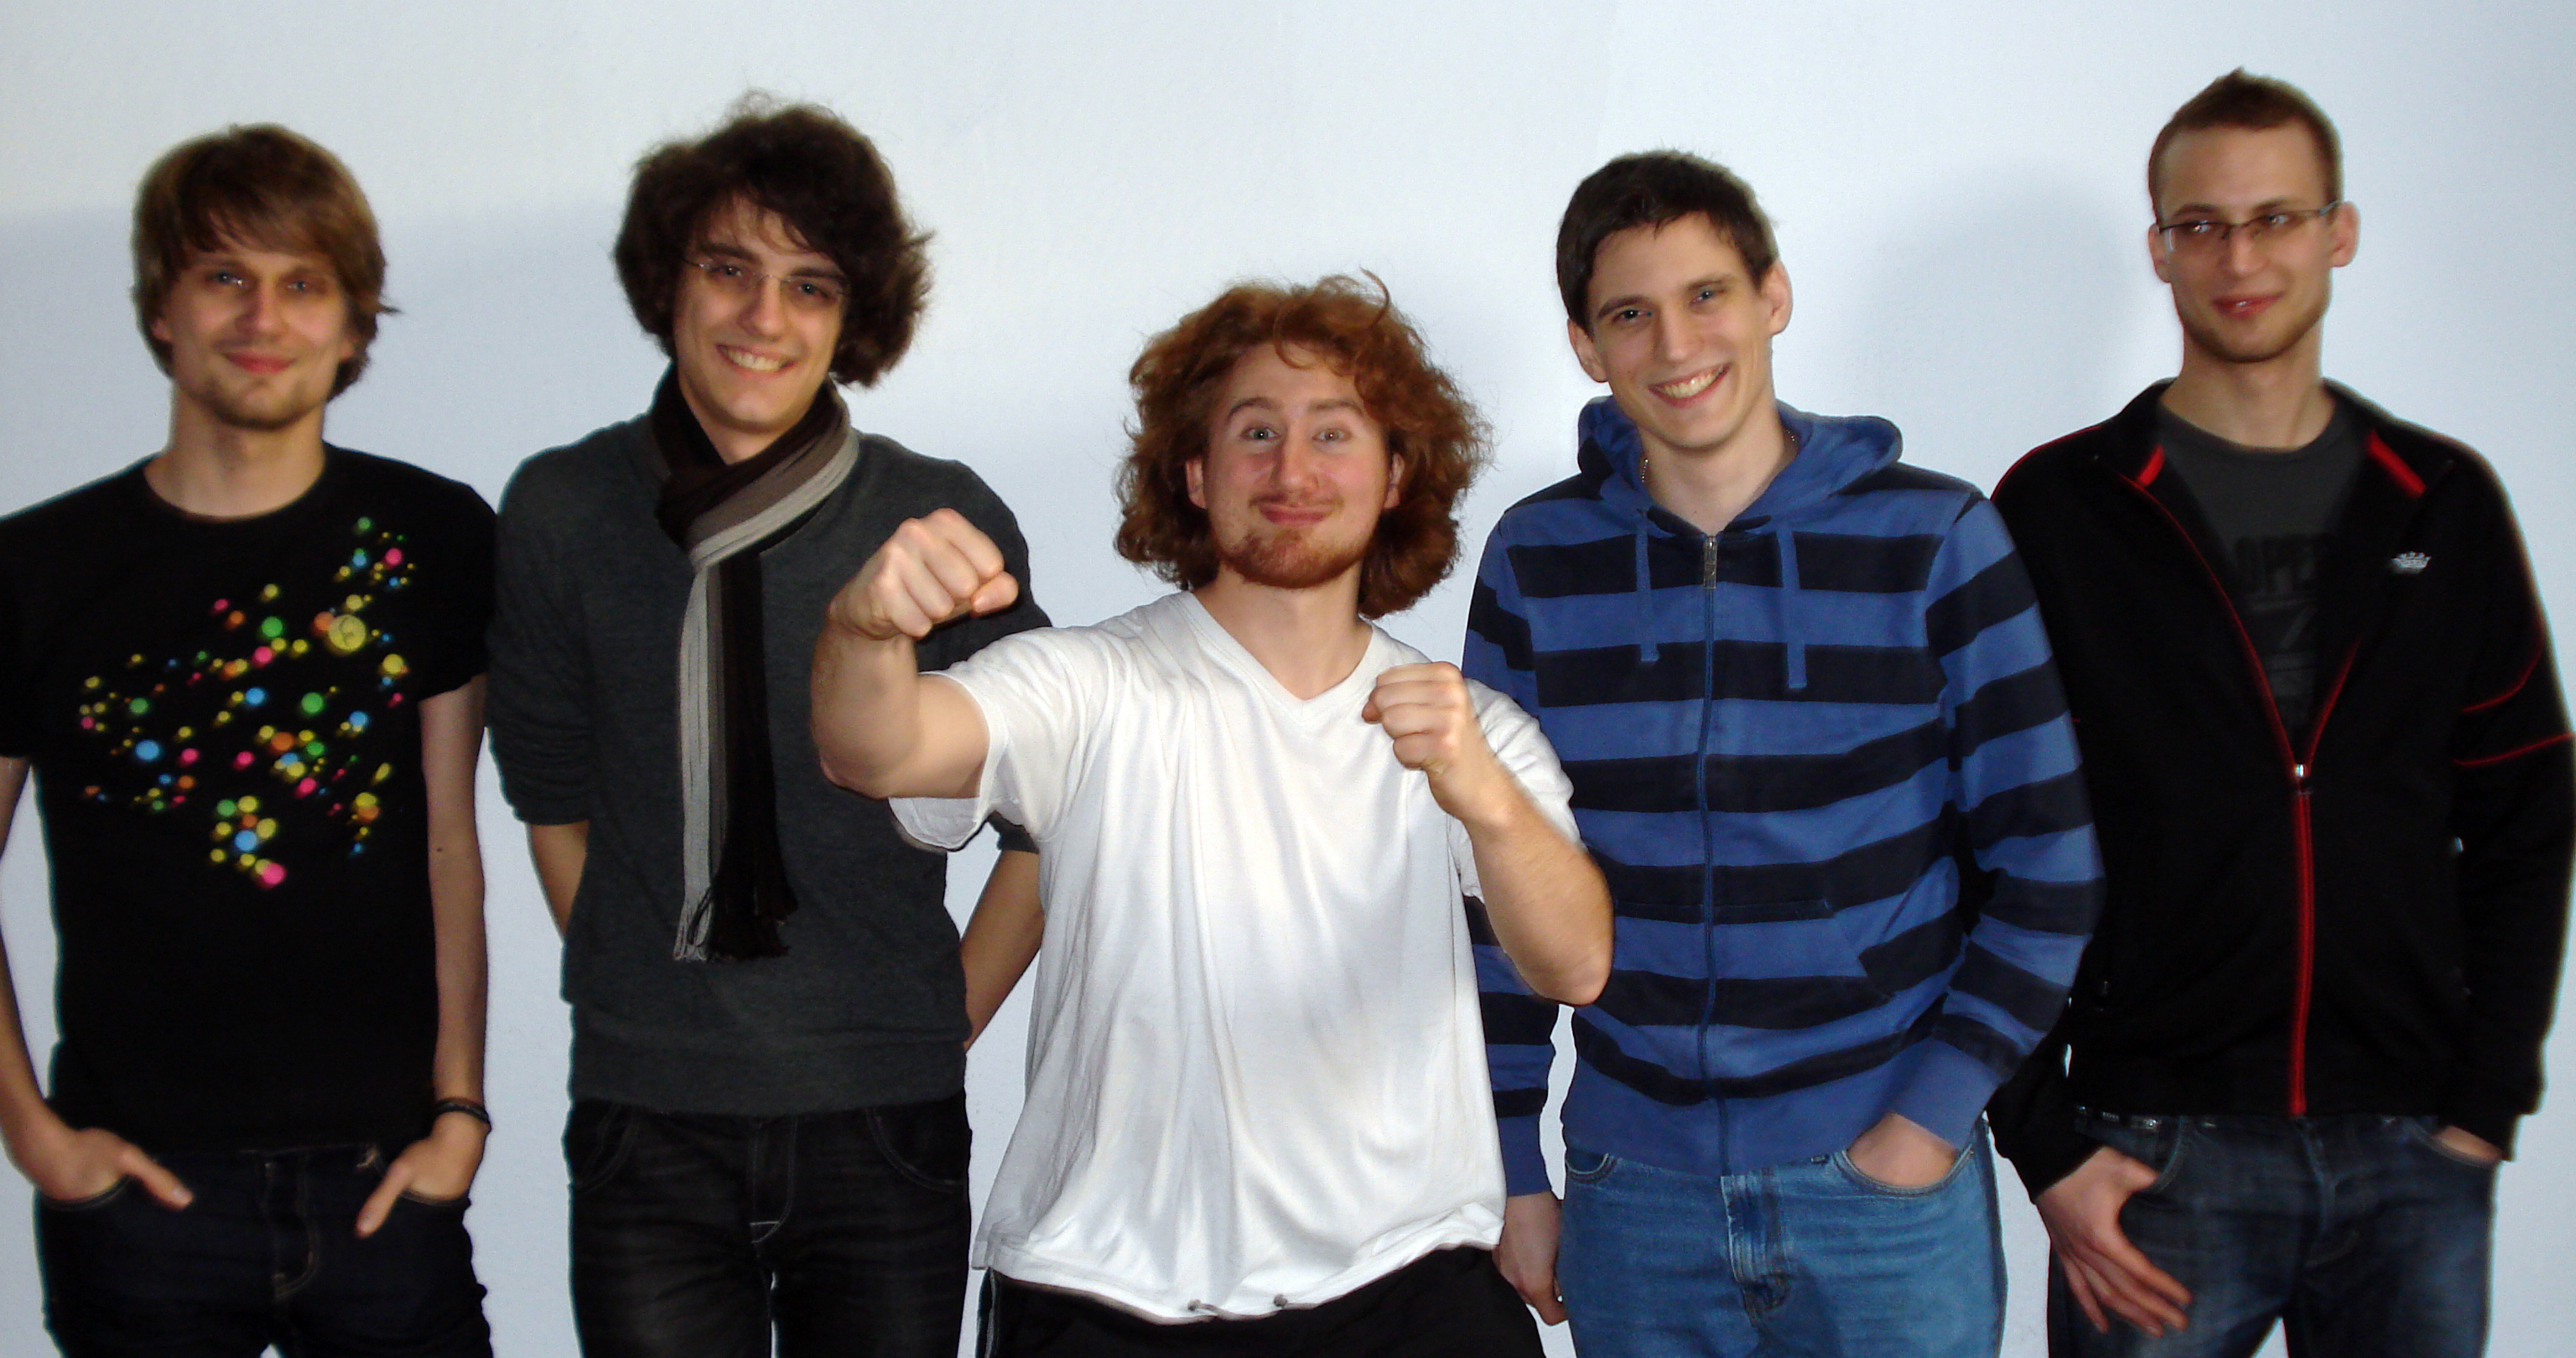
\includegraphics[width=\columnwidth]{images/team.jpg}
	\caption{\small From left to right: Andre Zoufahl, Konrad Reiche, Julian Fleischer, David Bialik, Hagen Mahnke}
	\label{fig:us}
\end{figure}

\end{multicols}
\begin{multicols}{2}[\section{Development process}]
\label{sec:development-process}

An important subfield of software engineering is the use of known methods and principles. The development process implies the used methods and principles. Thus this section will cover the chosen development process, its ideal procedure and how the development process actual took place including a timeline of events.

\end{multicols}
\begin{multicols}{2}[\subsection{Intended development process}]
\label{sec:intended-development-process}

As mentioned above \emph{MyCourses} is the first software project for everyone in the team. The selection of a development process was heavily based on the software engineering course we heard in the summer 2010. A major part of the project was realized in the period of lectures. This and the long distances between our homes is why we decided against an agile development process, as we did not have the opportunity to communicate and meet on a daily basis.

For the intended development process we chose the spiral model \cite{spiral}. An iterative model used incrementally seemed to be promising. Dividing our project into iterations would give us a frame of orientation for the project management. The incremental working method was fitting as we were sure there will be no functioning version of the program after the first iteration. Overall the spiral model focuses on solving those problems which reduce the projects risks at best. This fact reflected our expected work habits to adressing those problems which are blocking the project accomplishment the most.

We rather chose the spiral model as the basis for our own process and assumed that adaption would become necessary. We did not, however, have a clear concept of what might require adaption and how said adaption might be realized. Further we discussed essentials which should support and promote our work-flow. Key components of our process were therefore:

\begin{itemize}
\item \ads{regular meetings} for coordination
\item communication via \ads{e-mail}
\item evaluation of every iteration
\item \ads{ticket system} for defining and monitoring tasks
\item \ads{wiki} for collaborative document creation
\end{itemize}

\end{multicols}

\pagebreak

\begin{figure}[t]
	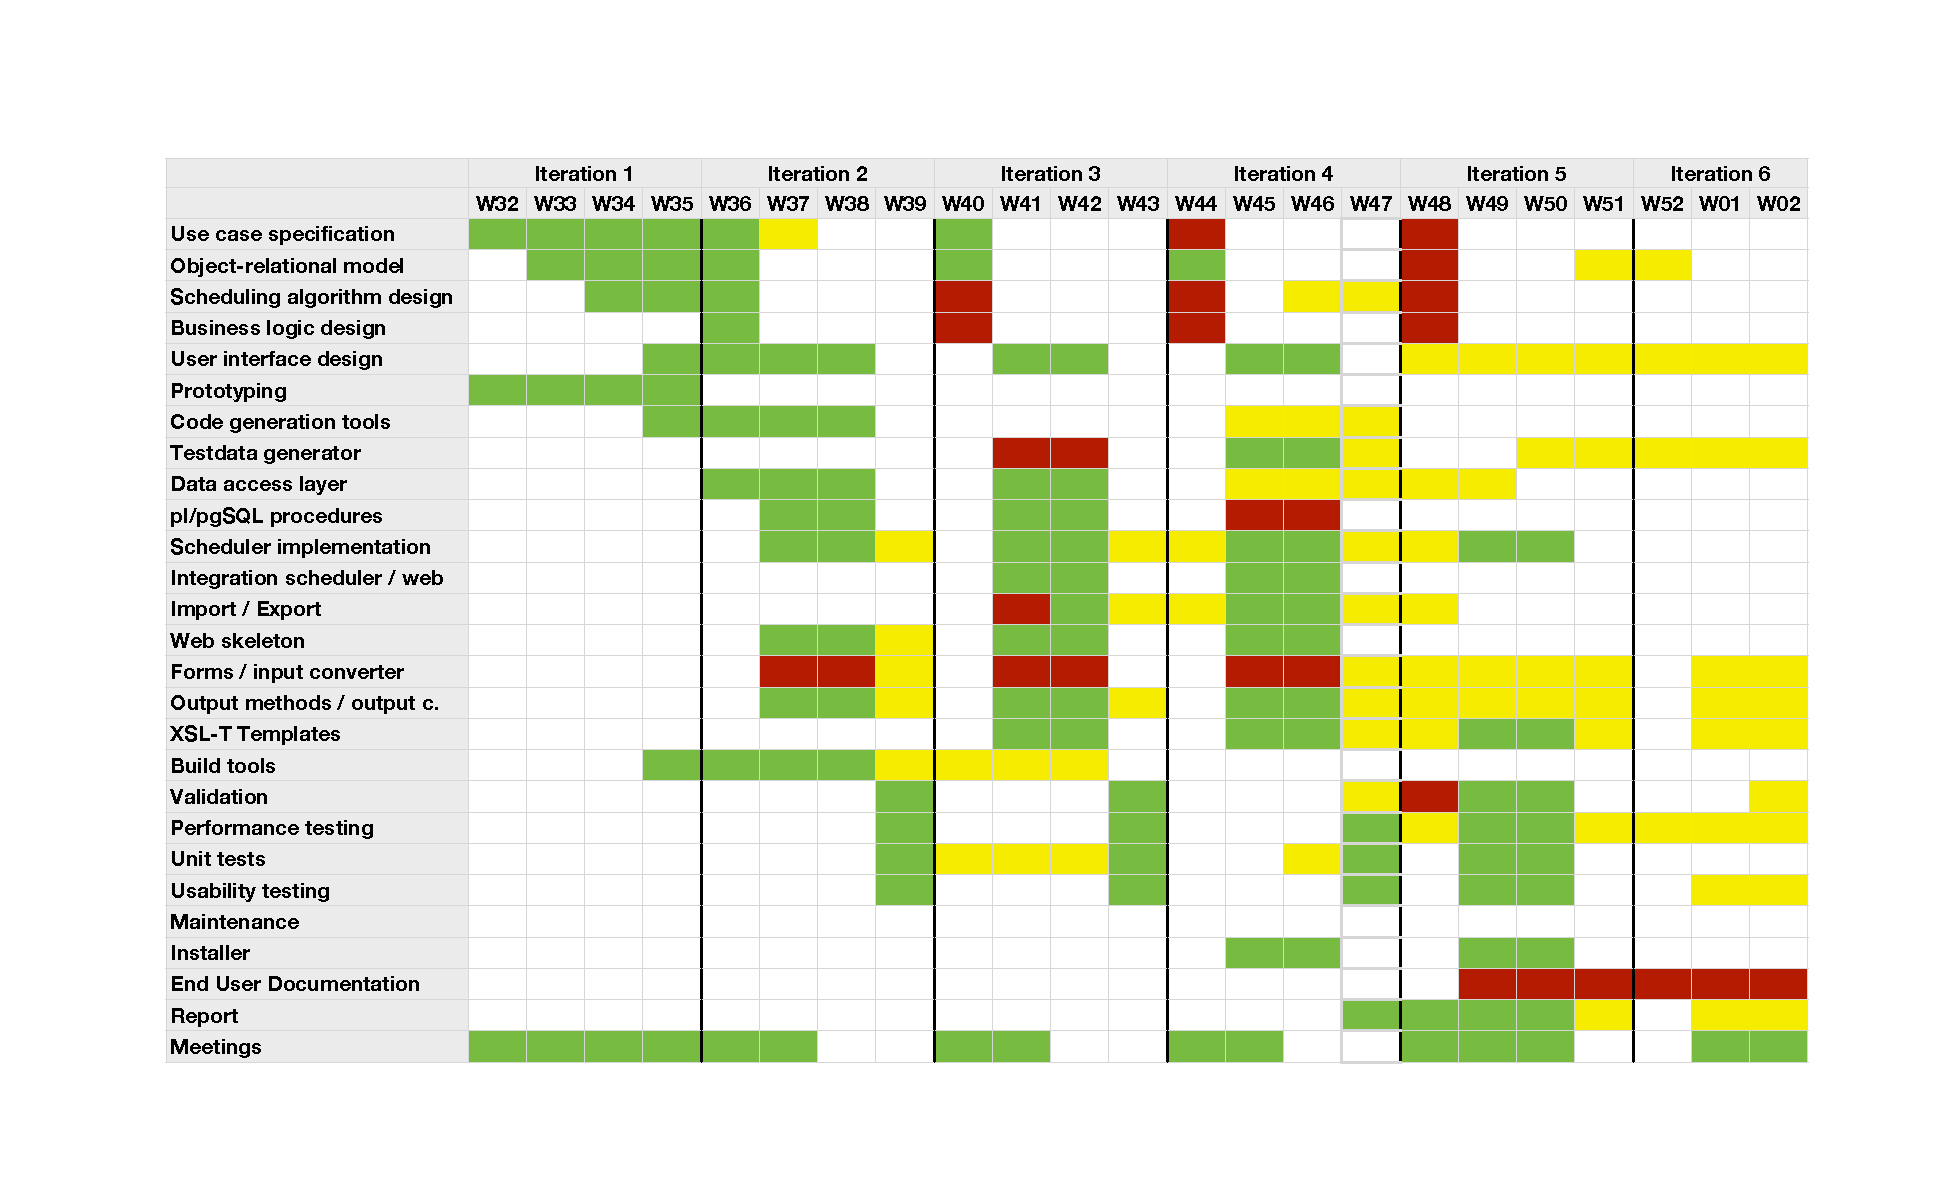
\includegraphics[width=\columnwidth]{images/gantt.pdf}
	{\color{YellowGreen} green} cells: components which we workend on as planned \\ {\color{Goldenrod} yellow} cells: components we worked on off our plan \\ {\color{BrickRed} red} cells: components we did not work on although planned
	\caption{Our project plan, originally conception and actual process}
	\label{fig:gantt-chart}
\end{figure}

\begin{multicols}{2}[\subsection{Actual development process}]
\label{sec:actual-development-process}

How the actual development process took place can be best understand when reading the timeline in section 2.3. In retrospect to the spiral model certain variations emerged. 

The beginning of every iteration is characterized by detailed requirement definitions. An intense requirement elicitation based on the \emph{MyCourses} specification was done in the first iteration with the result of a set of written use cases. In subsequent iterations, however, the requirement refinement was not done in the beginning of each iteration, but distributed over the iterations whenever problems with the current design emerged.

Even though we implemented a minimalistic prototype of \emph{MyCourses} in iteration 1, there was no continuous prototype development for comparation and evaluation as proposed by the spiral model. We focused on incremental development of the final product in every iteration.

In contrast other procedures in the development process went according to the spiral model. We put a lot of effort into the evaluation of different architectures and their resulting design. Further we tried to reduce the possible project risks by prioritizing the next main goals for the iteration.

In matters of organizing ourselves and use of methods we had a steep learning curve. In August and September we selected superordinated goals, but in the middle of each iteration we often lost focus of important tasks. The biggest improvement of the development process was therefore the introduction of weekly task assignments for every team member starting in October. Based on that, the tasks and their results were evaluated in every week, which lead to a purposeful work and swift discussion of emerging problems.



\end{multicols}
\begin{multicols}{2}[\subsection{Timeline}]
\label{sec:Timeline}
A short overview of the course our project took will be given in the next paragraphs. The goals for a phase were defined after evaluation of the previous phase had been completed. Before our project really started we got to know each other and decided which professor should be our contact person at university.

\begin{description}
\item[The First iteration] started on June 20, comprising an initial requirement elicitation, design of our software, prototyping of the scheduler and choosing technologies. During most of this time the academic term was still running and only a fraction of our time was devoted to the project. This iteration ended on September 9 and was evaluated the day before. Much of the time spent in this iteration was still focused on gaining orientation. Still it was necessary for us to take this time and find a suitable approach to the work ahead.

\item[The Second iteration] started on September 10 and was devoted to producing the scheduling algorithm, the web interface and our ORM as well as the servlet code. Work cycles were short and meetings were held every few days, including a weekend  devoted to coding. From this point on our iterations were reduced to about one month each, the focus being shifted on implementing and testing. Requirements and design were refactored whenever we felt the need to -- due to new insights or problems. This iteration ended on October 4 and was evaluated the same day.

\item[The Third iteration] accordingly started on October 5, but most work was halted until October 16 due to exams and all-day courses at university. Beginning with October 26 weekly two-hour meetings were held at our university during which everyone reported achievements and problems of the previous week. At the end of each session goals for the following week were set. These weekly meetings have proven to be a good way of coordinating work as well as motivating each other, so they were maintained for the remainder of the project. The main goal and achievement of this iteration was the integration of the scheduler with the web-interface and the connection to the database. Due to this employment of parts of our software many issues were found and fixed. Accordingly we shifted our focus further towards unit-testing and started using a tool to measure code coverage, that is how much of our code is actually being executed  as part of a unit-test. At the same time more  functionality was added to the web-interface. This iteration ended on November 1 and was evaluated the day before.

\item[The Fourth iteration] started on November 2, with the primary focus lying on the improvement of our web interface, adding functionality and a unified design. Several improvements to the scheduler algorithm were made, most notably the introduction of a greedy algorithm. Work on the summary report was also started during this iteration and the first version -- which was the basis for all further versions -- was written. The iteration ended on December 5.

\item[The Fifth iteration] started on December 6 and was mainly devoted to minor improvements to the scheduler and writing the beta-version of our summary report. One improvement to our database-access-layer which made query-caching available drastically improved scheduling performance by a factor of 8. The iteration ended on December 30.


\item[The Sixth iteration] was not part of our original project plan. The project was late and so we had to add three additional weeks for last feature implementations amd quality assurance.

\end{description}

\end{multicols}
\begin{multicols}{2}[\section{Requirements}]
\label{sec:requirements}
The following three sections are an overview of the problem and the resulting requirements. The first section  states the problem, while the second describes the elicitation we deduced from it, followed by the specification in the third section.

\end{multicols}
\pagebreak
\begin{multicols}{2}[\subsection{Problem statement}]

Organizations like universities and schools have to allocate courses to the given resources in a sensible way. As the amount of resources and courses grows large, it gets increasingly costly to do the allocation manually. Furthermore the task of course scheduling is repeated quite often and thus a lot of work is spent on it. Often the courses and resources remain consistent each term and large parts of the previous solution can be reused. Each solution to such a problem must satisfy a number of constraints.

\end{multicols}
\begin{multicols}{2}[\subsection{Requirement elicitation}]
\label{sec:requirement-elicitation}
Most of the requirements are already outlined in the project description of \emph{MyCourses}. Still we considered it helpful to get more insights into these requirements. To make the requirements more specific and better understood we created use cases. These use cases helped us during implementation as they provided an important frame of orientation.

As we also desired more insight into how a scheduling process might look like, we asked an employee of our institute to give us a demonstration. The demonstration was conducted on the system used at our institute. Although it did not reveal  completely unknown aspects to us, it gave us a better estimation of the importance of certain aspects.


\end{multicols}
\begin{multicols}{2}[\subsection{Requirement specification}]
\label{sec:requirement-specification}
The ideal scenario is a program that automatically finds an optimal solution. However the problem is NP-hard \cite{JSSP} and thus a computer-aided scheduling process is the focus.

The problem of course scheduling is defined by the given constraints which have to be satisfied. In order to meet the \emph{MyCourses} specification requirements of high configurability we distinguish constraints by \emph{hard} and \emph{soft constraints}.

\begin{description}
\item[Hard constraints] are constraints which must be satisfied. If these constraints are not satisfied the lecturing of courses is not possible. This includes the following constraints:

\begin{itemize}
\item not more than 1 course in the same room at the same time

\item the course lecturer teaches no other course at the same time

\item courses belonging to the same year do not overlap with each other in time in order to ensure studiability

\item every constraint defined by the user with the priority of $100\%$, for instance preferred time, preferred room, etc.
\end{itemize}

\item[Soft constraints] are constraints which need not to be ultimately satisfied. This includes only constraints defined by the user with a priority less than $100\%$.
\end{description}

An \emph{optimal solution} is a scheduling which asserts the satisfaction of all \emph{hard} and \emph{soft} constraints.


As the interests of many employees and students at the universities are affected by the result, they should be allowed to participate in the process or at least be taken into consideration. The requirements that had the greatest influence on our initial design and each subsequent change are:

\begin{itemize}
	\item automatic and manual allocation of courses
	\item satisfaction of hard and softconstraints
	\item suited for multi-user environments
	\item scalable scheduling
	\item defining/ presenting of scheduling-related information
	\item user-friendly look and feel
	\item access restriction to different areas
\end{itemize}


\end{multicols}

\pagebreak
\begin{multicols}{2}[\section{Architecture}]

\label{sec:architecture}

The following section will briefly overview the architecture of our software.

\end{multicols}
\begin{multicols}{2}[\subsection{Overview}]
\label{sec:architecture-overview}

Early on we divided our software into two major components, which – seen individually – should be able to run as stand alone applications as well as as integrated components. This approach should give us the ability to work on different parts of the software more independently. Furthermore, since both components are largely decoupled, it would be easier changing one of them without breaking the other.

These two components are:
\begin{description}
\item[A scheduler] which provides for an automatic allocation of courses to rooms and times.
\item[A web application] which is splitted into three tiers:
	\begin{itemize}
	\item The front end
	\item A controlling unit \emph{(controller)}
	\item The business logic
	\end{itemize}
\end{description}

Both components should work on common ground, which emerges naturally from the need for both to work on the same data. Thus they were to access the same database and we decided to create a data access layer which should be shared by both components.

\begin{figure}[H]
	\centering
		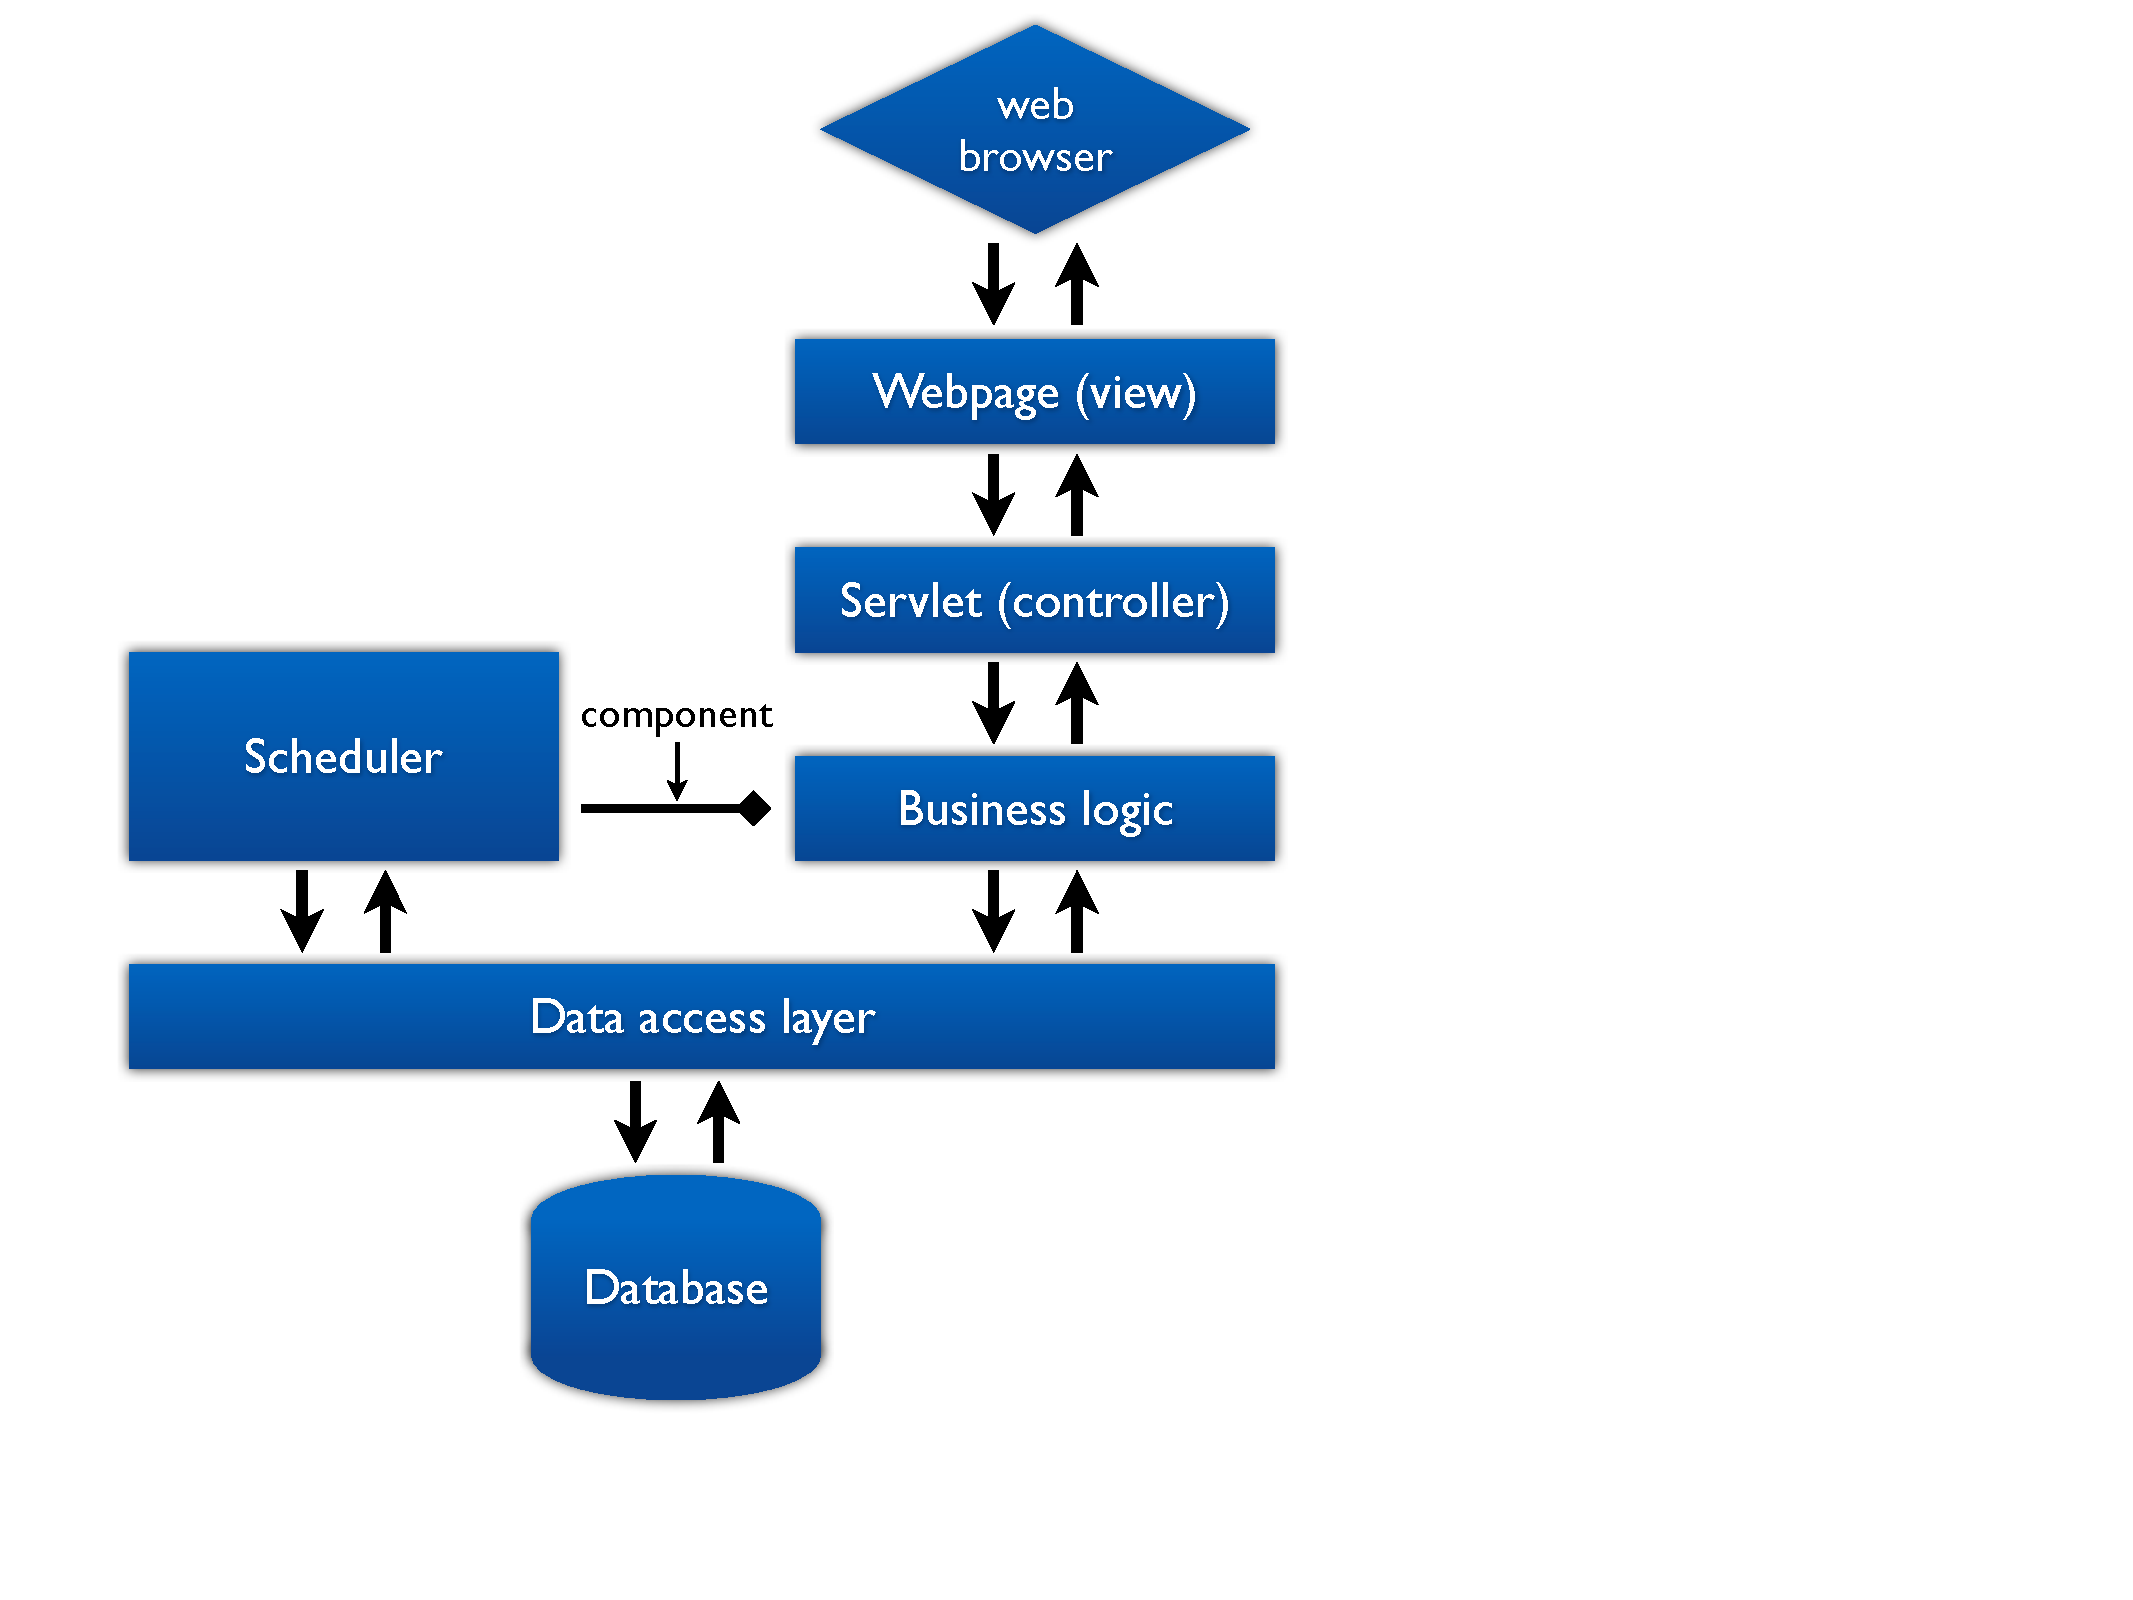
\includegraphics[width=\columnwidth]{images/architecture.pdf}
		\caption{An overview of the components}
	\label{fig:architecture}
\end{figure}


\end{multicols}
\begin{multicols}{2}[\subsection{Data access layer}]
\label{sec:architecture-data-access-layer}

In order to create a proper model of the entities we were to work with, we decided to develop an object-relational model. By that we understand a model which can easily be mapped to an object-oriented model, as well as an entity-relationship-model\footnote{Not to be confused with approaches to store objects in relational databases} from which the object-oriented classes as well as an entity-relationship database definition can be derived.

\begin{figure}[H]
	\centering
		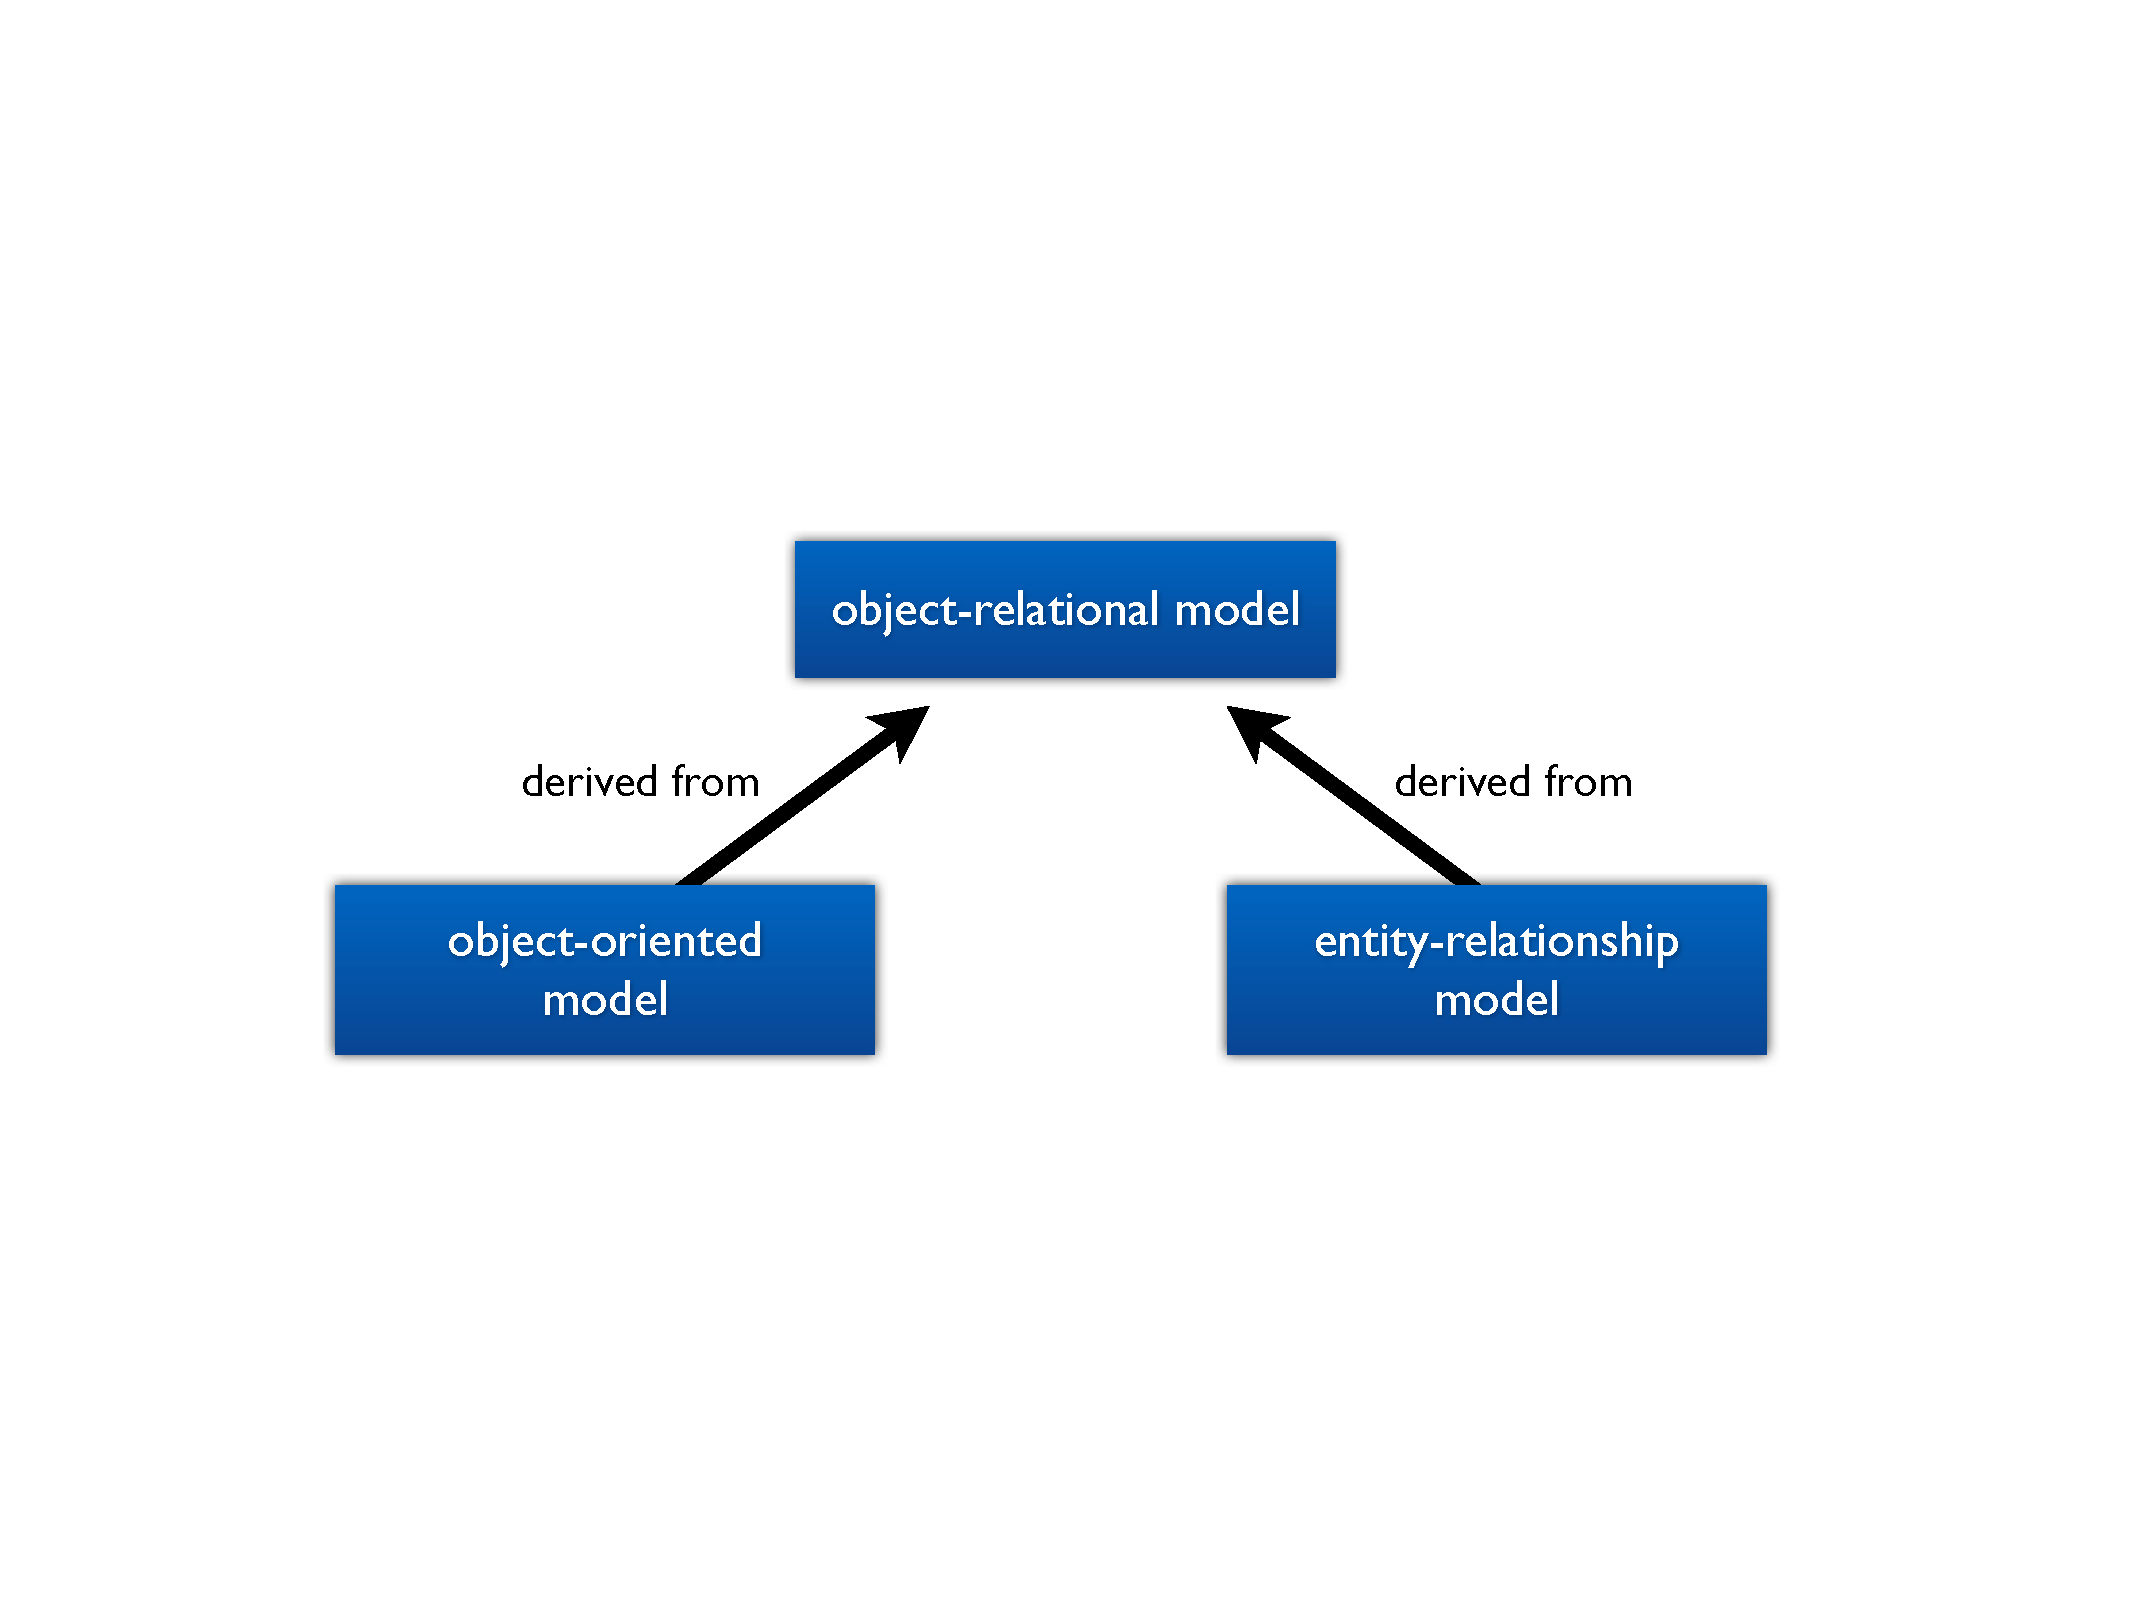
\includegraphics[width=\columnwidth]{images/model.pdf}
		\caption{The object-oriented model and the entity-relationship oriented model are derived from the object-relational model. Since both the OO as well as the ER model derive from the same basic model, they are guaranteed to be in a consistent state.}
	\label{fig:model}
\end{figure}


\end{multicols}
\begin{multicols}{2}[\subsection{Scheduler}]

For providing a reasonably fast pre-scheduling, we wanted to use a genetic algorithm. Such algorithms roughly consist of three parts:

\begin{description}
\item[A fitness function] which evaluates the quality of an intermediate solution.

\item[A cross over function] which intermixes two intermediate solutions in a specific manner in order to create a better solution.

\item[A mutation function] which randomly or intelligently refactors an intermediate solution.

\item[The algorithm itself] which controls the execution of the other parts, i.e. in what order the components are applied and how many intermediate solutions are created.

\end{description}

We decided to model these parts as exchangable components, i.e. individual objects, which could be combined in any way. Since we did not have any experience with these kind of algorithms this design should help us to better understand and scale the different parts of the algorithm.

\label{sec:architecture-scheduler}



\end{multicols}
\begin{multicols}{2}[\section{Technologies}]
\label{sec:technologies}

Since our design was heavily influenced by the technologies we wanted to use, we will give a brief discussion of the technologies we used and why we chose to use them.

We considered many technologies and looked at some of them intensively. Since we were building a web application we considered PHP, Ruby, Scala, pure Java and AspectJ as our main programming language. As the scheduler is a performance critical part of our application we dropped interpreted languages early. As we were all most familiar with Java and development tools for Java are widely available, we favored Java. We finally went with \ads{AspectJ}\link{http://www.eclipse.org/aspectj}{The eclipse AspectJ project}, which is built on top of Java, since it offers great flexibility through so called Aspects. It is tightly integrated in our favored IDE\footnote{Integrated Development Environment}, Eclipse, since it is an Eclipse project itself. We will discuss the use of Aspects within our application more in-depth later on.

As database backend we chose \ads{PostgreSQL}\link{http://www.postgresql.org/}{PostgreSQL} since it features strong adherence to the SQL standard and is the best open source implementation of \emph{referential integrity} in relational databases we knew of. Another strong argument for PostgreSQL was, that it allows for rich use of stored procedures, i.e. business logic within the database. As a matter of fact our application thus runs with PostgreSQL only, but could be ported to another database-engine easily, since only certain parts would have to be rewritten (PostgreSQL-specific parts within the data access layer and certain Aspects).

We used the standard web technologies like \ads{HTML}\link{http://www.w3.org/html/}{W3C HTML homepage} and \ads{CSS}\link{http://www.w3.org/Style/CSS/}{W3C Cascading StyleSheets homepage} in the front end. To keep things simple we stuck to related technologies which are all part of the \ads{XML family}, like \ads{XSL-T}\link{http://www.w3.org/TR/xslt}{XSL Transformations (XSLT)}. We will disucss the use of XML within our web application in the appropriate sections of this report.


\end{multicols}
\begin{multicols}{2}[\subsection{Libraries \& Frameworks}]
\label{sec:libraries-and-frameworks}

In order to enrich users experience, we made use of \ads{jQuery}\link{http://www.jquery.org}{Homepage of jQuery}. However, in order to keep the site accessible, we did not use it too much, i.e. the site should be fully functionial even if JavaScript was deactivated.

On the backend side we employed many libraries from the Apache Software Foundation, namely from their XML Software Stack. Amongst others, these are \ads{Apache Xalan}\link{http://xalan.apache.org}{Apache Xalan XSL-T Processor} and \ads{Apache FOP}\link{http://xmlgraphics.apache.org/fop/}{Apache XSL-FO Processor}, which we used to process XSL and generate not only XHTML, but also PDF files.

To create an easy to use installer we used \ads{IzPack}\link{http://www.izpack.org/}{Homepage of IzPack}. To make sure that our application works with different application servers it can optionally be bundled with Jetty\link{http://www.eclipse.org/jetty/}{Jetty Web Server} (an embedabble servlet container), which itself also is an Eclipse project.


\end{multicols}
\begin{multicols}{2}[\subsection{Tools}]
\label{sec:tools}

As mentioned in \autoref{sec:development-process}, we made use of a wiki and a ticket system. Both of them are contained in \ads{Trac}\link{http://trac.edgewall.org}{The Trac project}, a webinterface to \ads{Subversion}\link{http://subversion.tigris.org/}{Subversion homepage}, which we both used for source and version control.

We used \ads{JUnit}\link{http://www.junit.org/}{JUnit Test Driven Development} for writing unit tests. For the automatic execution of this, as well as generating reports about line coverage and branch coverage, we used \ads{Cobertura}\link{http://cobertura.sourceforge.net/}{Cobertura – Code coverage analysis tool}.

To build our project, we used GNU Make initially, but later on we switched to \ads{Apache Ant}, since it is more platform independent and features plugins which tightly integrate with AspectJ and JUnit. For testing purposes we employed \ads{Apache Tomcat}.

Regarding the versions of mentioned tools we followed the policy to include nothing more recent than the latest stable version of the Debian GNU/Linux distribution.


\end{multicols}
\begin{multicols}{2}[\subsection{Code generation toolbox}]
\label{sec:toolbox}

As we mentioned in \autoref{sec:architecture}, we did not want to maintain separate models for our database and our application. To achieve this technically we created an XML-file which represented an abstract description of our object-relational model. The syntax and semantics were defined using XML Schema\link{http://www.w3.org/XML/Schema}{XML Schema}. Using different XSL-T Stylesheets we automatically generated Java source files, an SQL install script, and documentation in XHTML.

As part of our build process we developed some tools for automatic generation of code. Basically the toolbox consists of several XSL-T stylesheets which can be used to create Java code, SQL scripts or XHTML documentation from a custom XML definitions file. This file contains the object-relational model and is specified using XML Schema.

The whole process of generating code is driven by Ant and part of our build process. Also the database can be easily set up using our toolchain.

\begin{figure}[H]
	\centering
		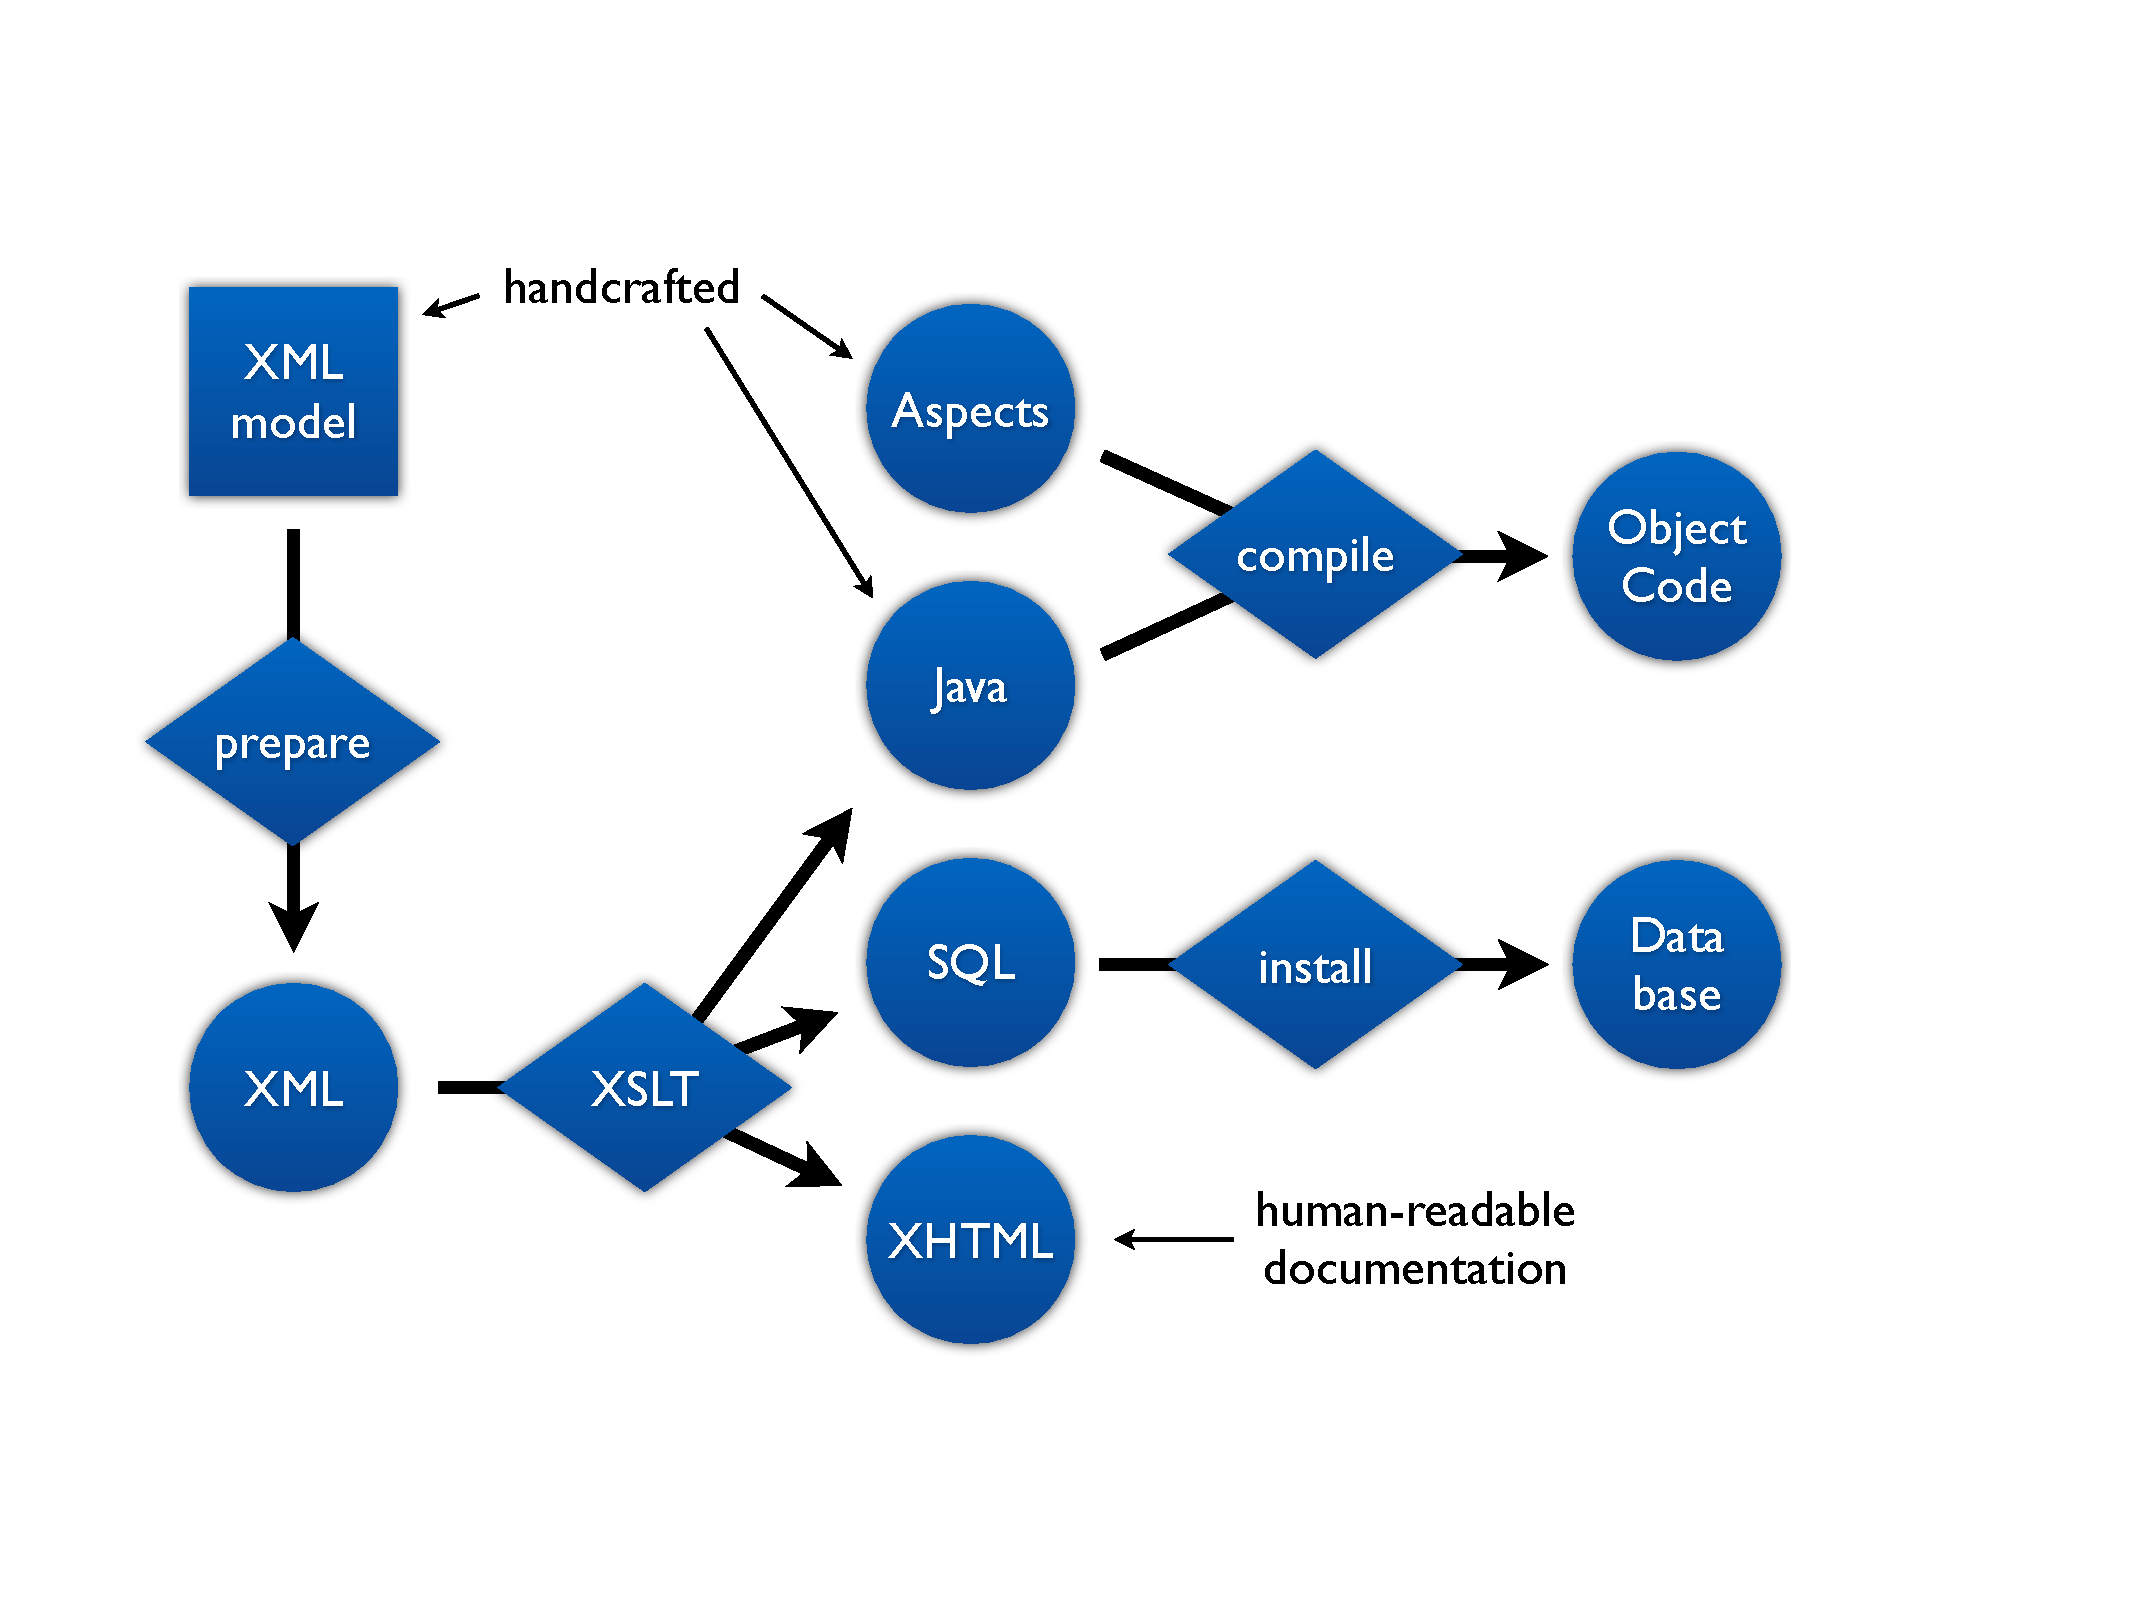
\includegraphics[width=\columnwidth]{images/build-process.pdf}
	\caption{The process of generating code within scetris.}
	\label{fig:build-process}
\end{figure}



\end{multicols}
\begin{multicols}{2}[\section{Design}]
\label{sec:design}

In the following subsections our design decisions are briefly explained. A description of how these influenced our project and what we learned from them will be given in the \autoref{sec:outcomes}. The first section discusses our domain model. The second section deals with our data access layer. The third section is about our web application. The last section describes the scheduler algorithm.

\end{multicols}
\begin{multicols}{2}[\subsection{Domain model}]

Since universities are organized quite differently we tried to design the domain model as generic as possible. An important aspect of the application is reusability of course definitions. This requirement lead to the following design of course related information in our domain model.

\begin{description}
	\item [Course] is a well-defined set of \emph{CourseElements} and has only a name. For example the department of physics offers the course Thermodynamics.
	\item [CourseElement] is part of a \emph{Course} with a type and a duration. The course Thermodynamics consists of two \emph{CourseElements}, a two-hour lecture and a four-hour workshop.
	\item [CourseInstance] is a realization of a course for a specific program. The course Thermodynamics is held every second academic term. 
	\item [CourseElementInstance] is a realization of a \emph{CourseElement}, where several \emph{CourseElementInstances} constitute one \emph{CourseElement}. For instance the lecture is held on Monday from 10 to 12. The workshop on the other hand is divided into two events, that are held on Tuesday from 10 to 12 and Friday from 8 to 10.
\end{description}

Universities differ in their definitions of class types, features that a room may or may not have and features that a course may require. As such it appears to be infeasible to predefine these properties appropriately. Therefore our model allows universities to define the possible values of these properties. This generic modelling of properties is achieved by representing them as an attribute in a special entity. These entities are connected to the original entity indirectly through a relation that defines the connection.

\begin{figure}[H]
	\centering
		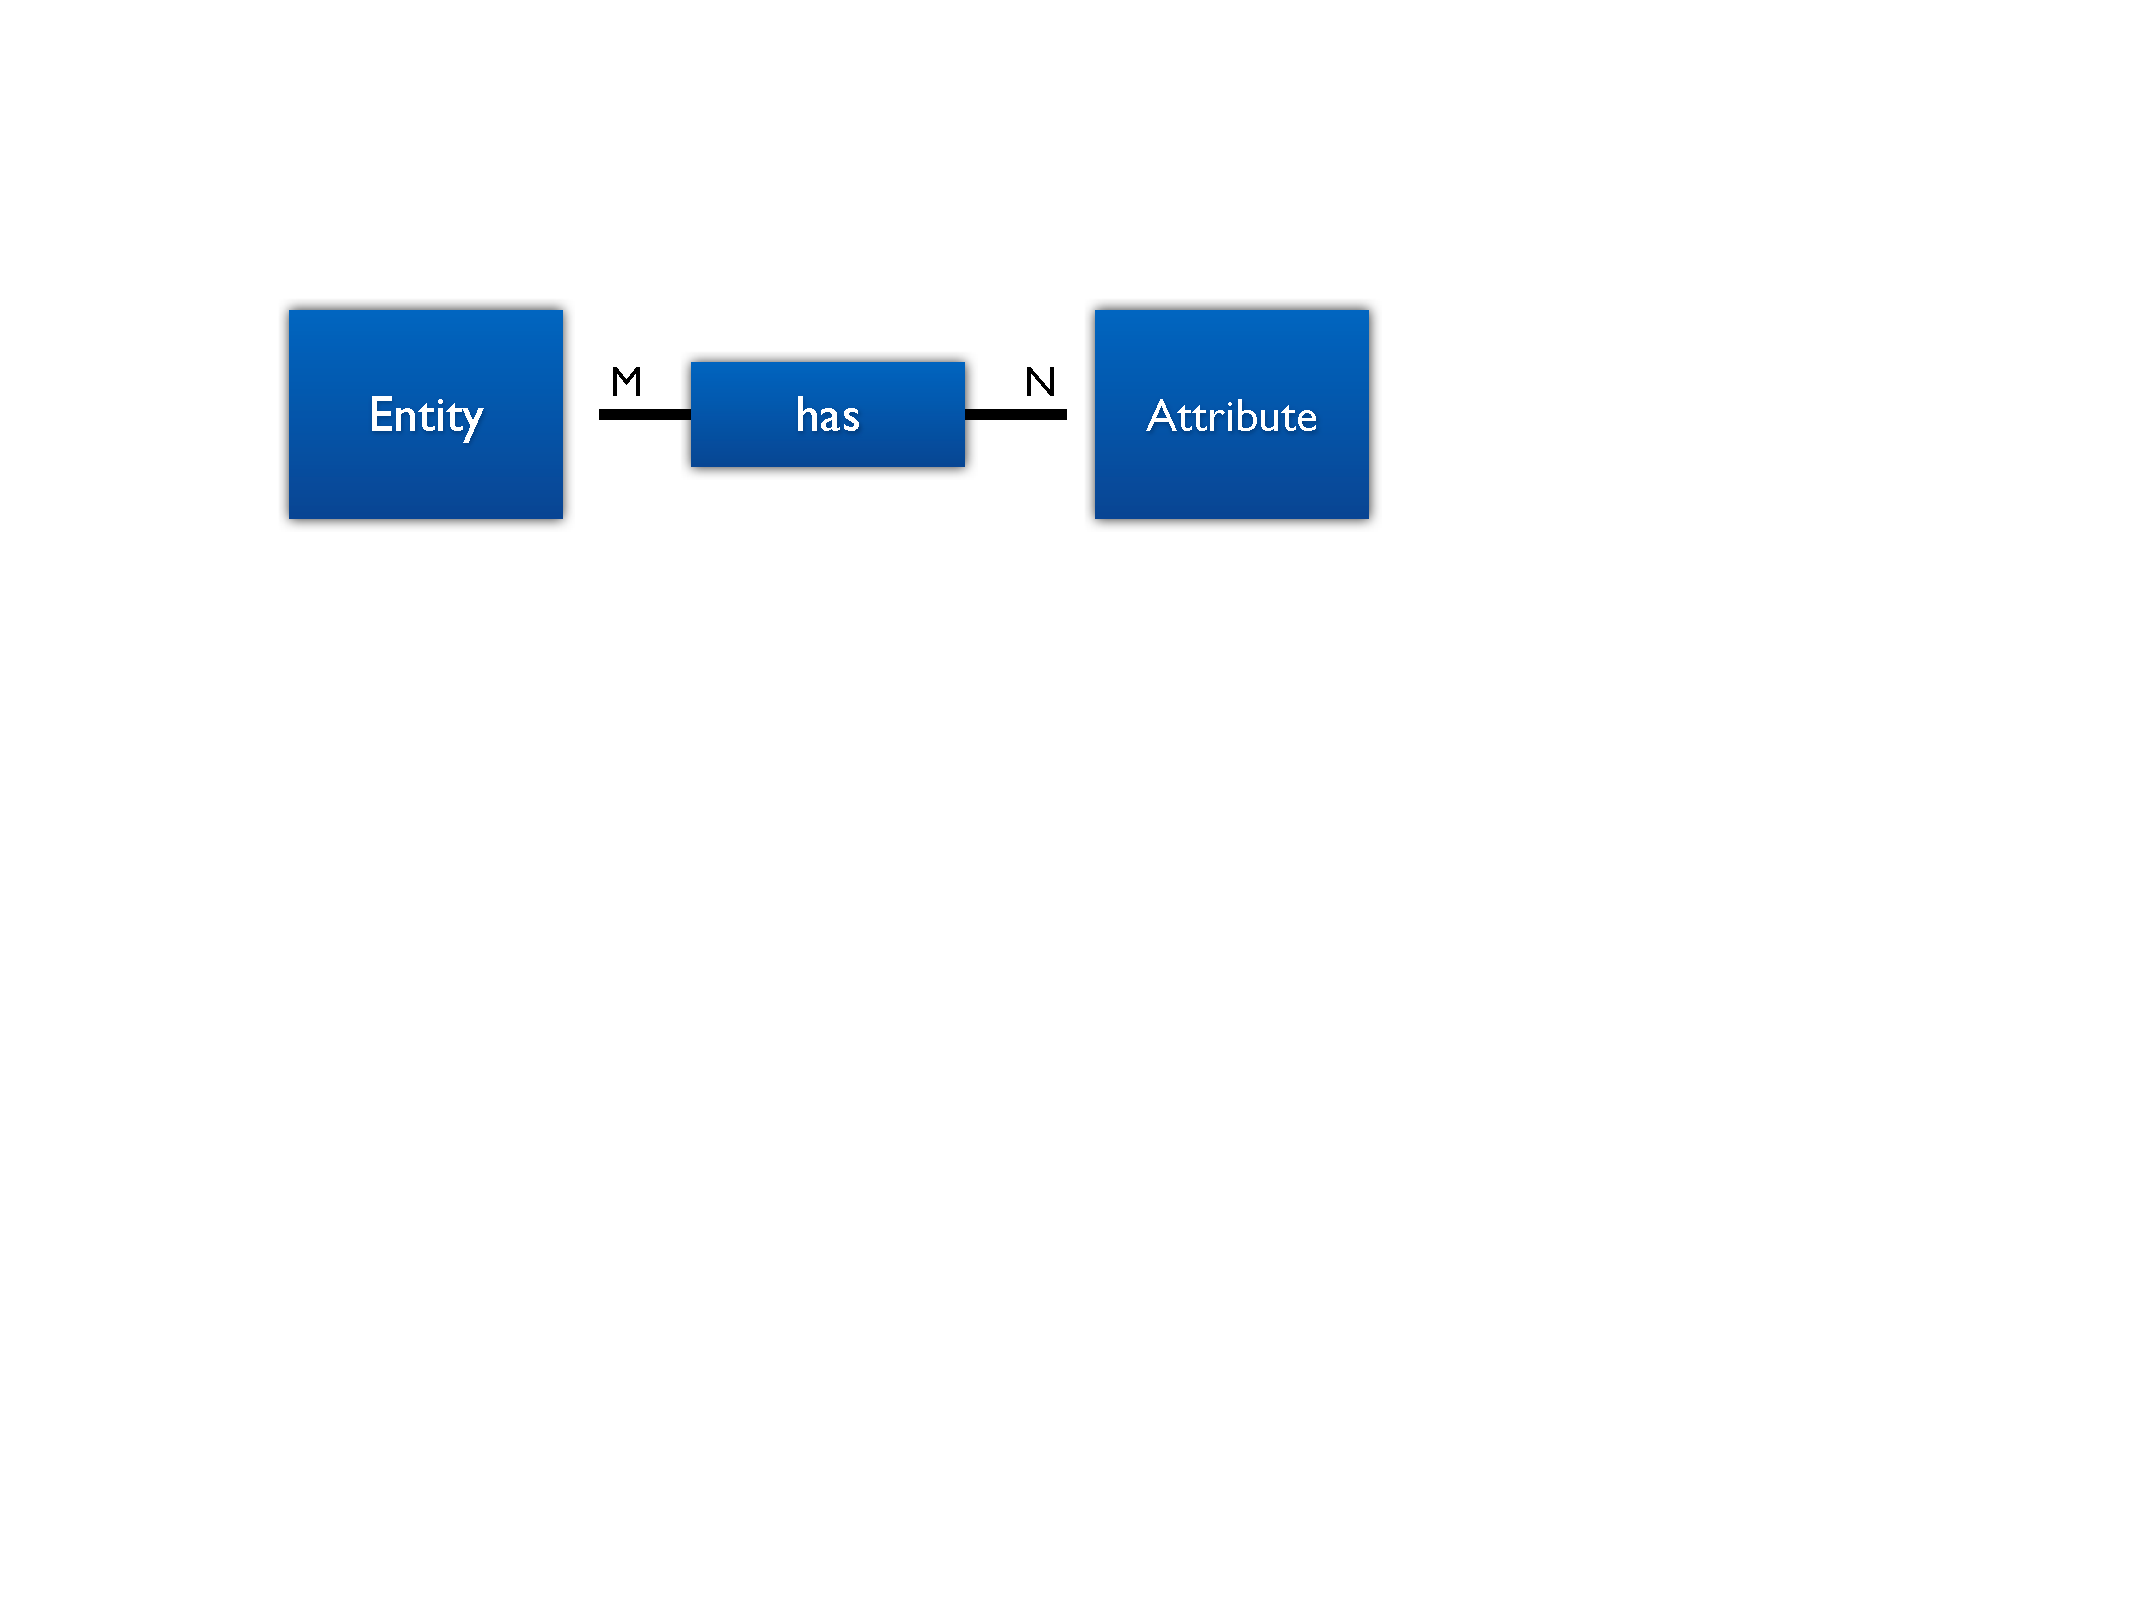
\includegraphics[width=\columnwidth]{images/orm_personroleprivilege.pdf}
	\caption{Many-to-many relation: generic model is achieved by representing them as an attribute in a
 special entity.}
	\label{fig:personroleprivilege}
\end{figure}

This also applies to user management where many different roles and sets of privileges are conceivable. Privileges themselves are predefined as they are a direct result of the possible actions. Furthermore universities might want to store additional information related to a course or person. The generic properties for Features of Rooms, CourseElements and CourseElementInstances are

\begin{itemize}
	\item CourseElement requires Feature
	\item CourseElementInstance requires Feature
	\item Room provides Feature
\end{itemize}

This means that for example a CourseElementInstance can have an arbitrary number of user defined Features. The connection is established through the relation CourseElementInstanceRequiresFeature. The connection can hold information about the minimum and maximum quantity, i.e. the number of seats a Room provides is represented in RoomProvidesFeature where the Feature has the name Seat.

\begin{itemize}
	\item Person has Attribute
	\item Course has CourseAttribute
\end{itemize}

Can be used to add user-defined attributes to a Person or a Course. For example the address of a Person can be stored as an Attribute.

\begin{itemize}
	\item Person has Role
	\item Role implies Privilege
	\item Person has Privilege
\end{itemize}

Are used by the user management to provide Privileges to groups  by RolImpliesPrivilege, or directly to Persons. For example the Role secretary may have user management Privileges. Furthermore the model enables a wide range of constraints.

\begin{itemize}
\item CourseElementInstance prefers Room

\item CourseElementInstance prefers Timeslot

\item Person prefers Timeslot

\item Room prefers Timeslot
\end{itemize}


\end{multicols}
\begin{multicols}{2}[\subsection{Data access layer}]

The object-relational model we defined deals with entities and relationships. Relationships connect two entities in a certain manner. Since they can have attributes too, we decided to model them as individual objects too, i.e. they are both represented as a table in the database as well as as a class in our object-oriented domain model. These classes implement the interfaces \emph{Entitiy} or \emph{Relationship} which in turn extend the interface Relation.

The objects should both represent the data as well as control the communication with the database, that means, they should be \emph{DAOs} (\emph{data access objects}) and \emph{DTOs} (\emph{data transfer objects}) at the same time. To accomplish this, we designed them as \emph{Active Records}. They feature methods to create, update and delete them. For retrieving data a special \emph{RelationManager} was defined. It is the central access point to the database and acts as a \emph{Factory} for the Active Records.

Since the code for the data access layer is auto generated its static structure follows a strict pattern. Each record has getters and setters to access the encapsulated data, the RelationManager has factory methods for each Entity and Relationship. Records that represent entities do also have special methods for retrieving datasets which are related via a special Relationship. One can now ask a Person-record which Privileges it has via PersonHasPrivilege-relationships, i.e. what the objects to the PersonHasPrivilege-relationship, in which that record is the subject, are. It is also possible to ask the other way around, i.e. what subjects are assigned to a given object via a certain relationship.

One key feature of the active records is, that if something (for example an attribute which represents a reference to another dataset) is requested which has not yet been retrieved from the database, it may transparently be fetched from the database. If, on the other hand, that record has already been fetched it may simply be loaded from a cache.

\begin{figure}[H]
	\centering
		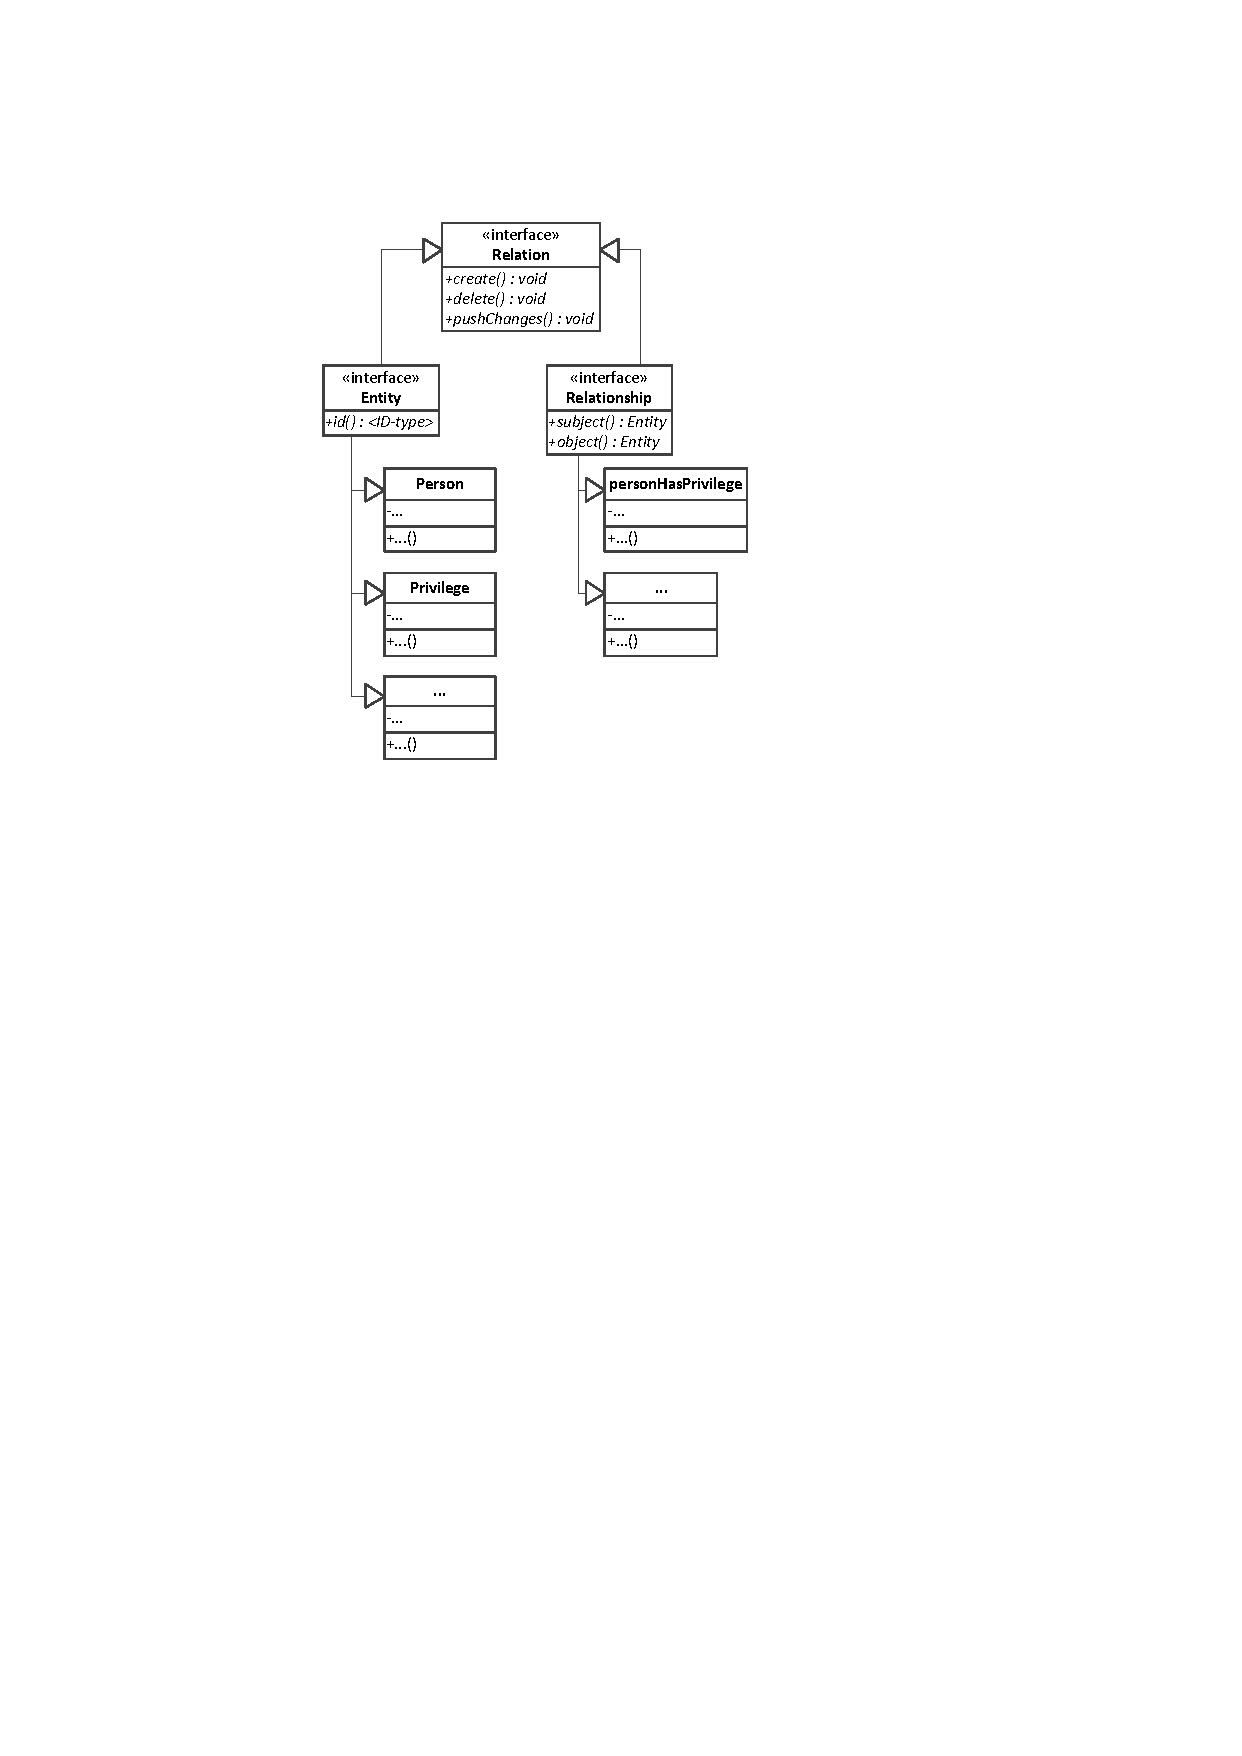
\includegraphics[width=\columnwidth]{images/UML-active-records.pdf}
	\caption{Overall structure of the active records}
	\label{fig:data-access-layer}
\end{figure}

\end{multicols}
\begin{multicols}{2}[\subsection{Web application}]

\begin{figure}[H]
	\centering
		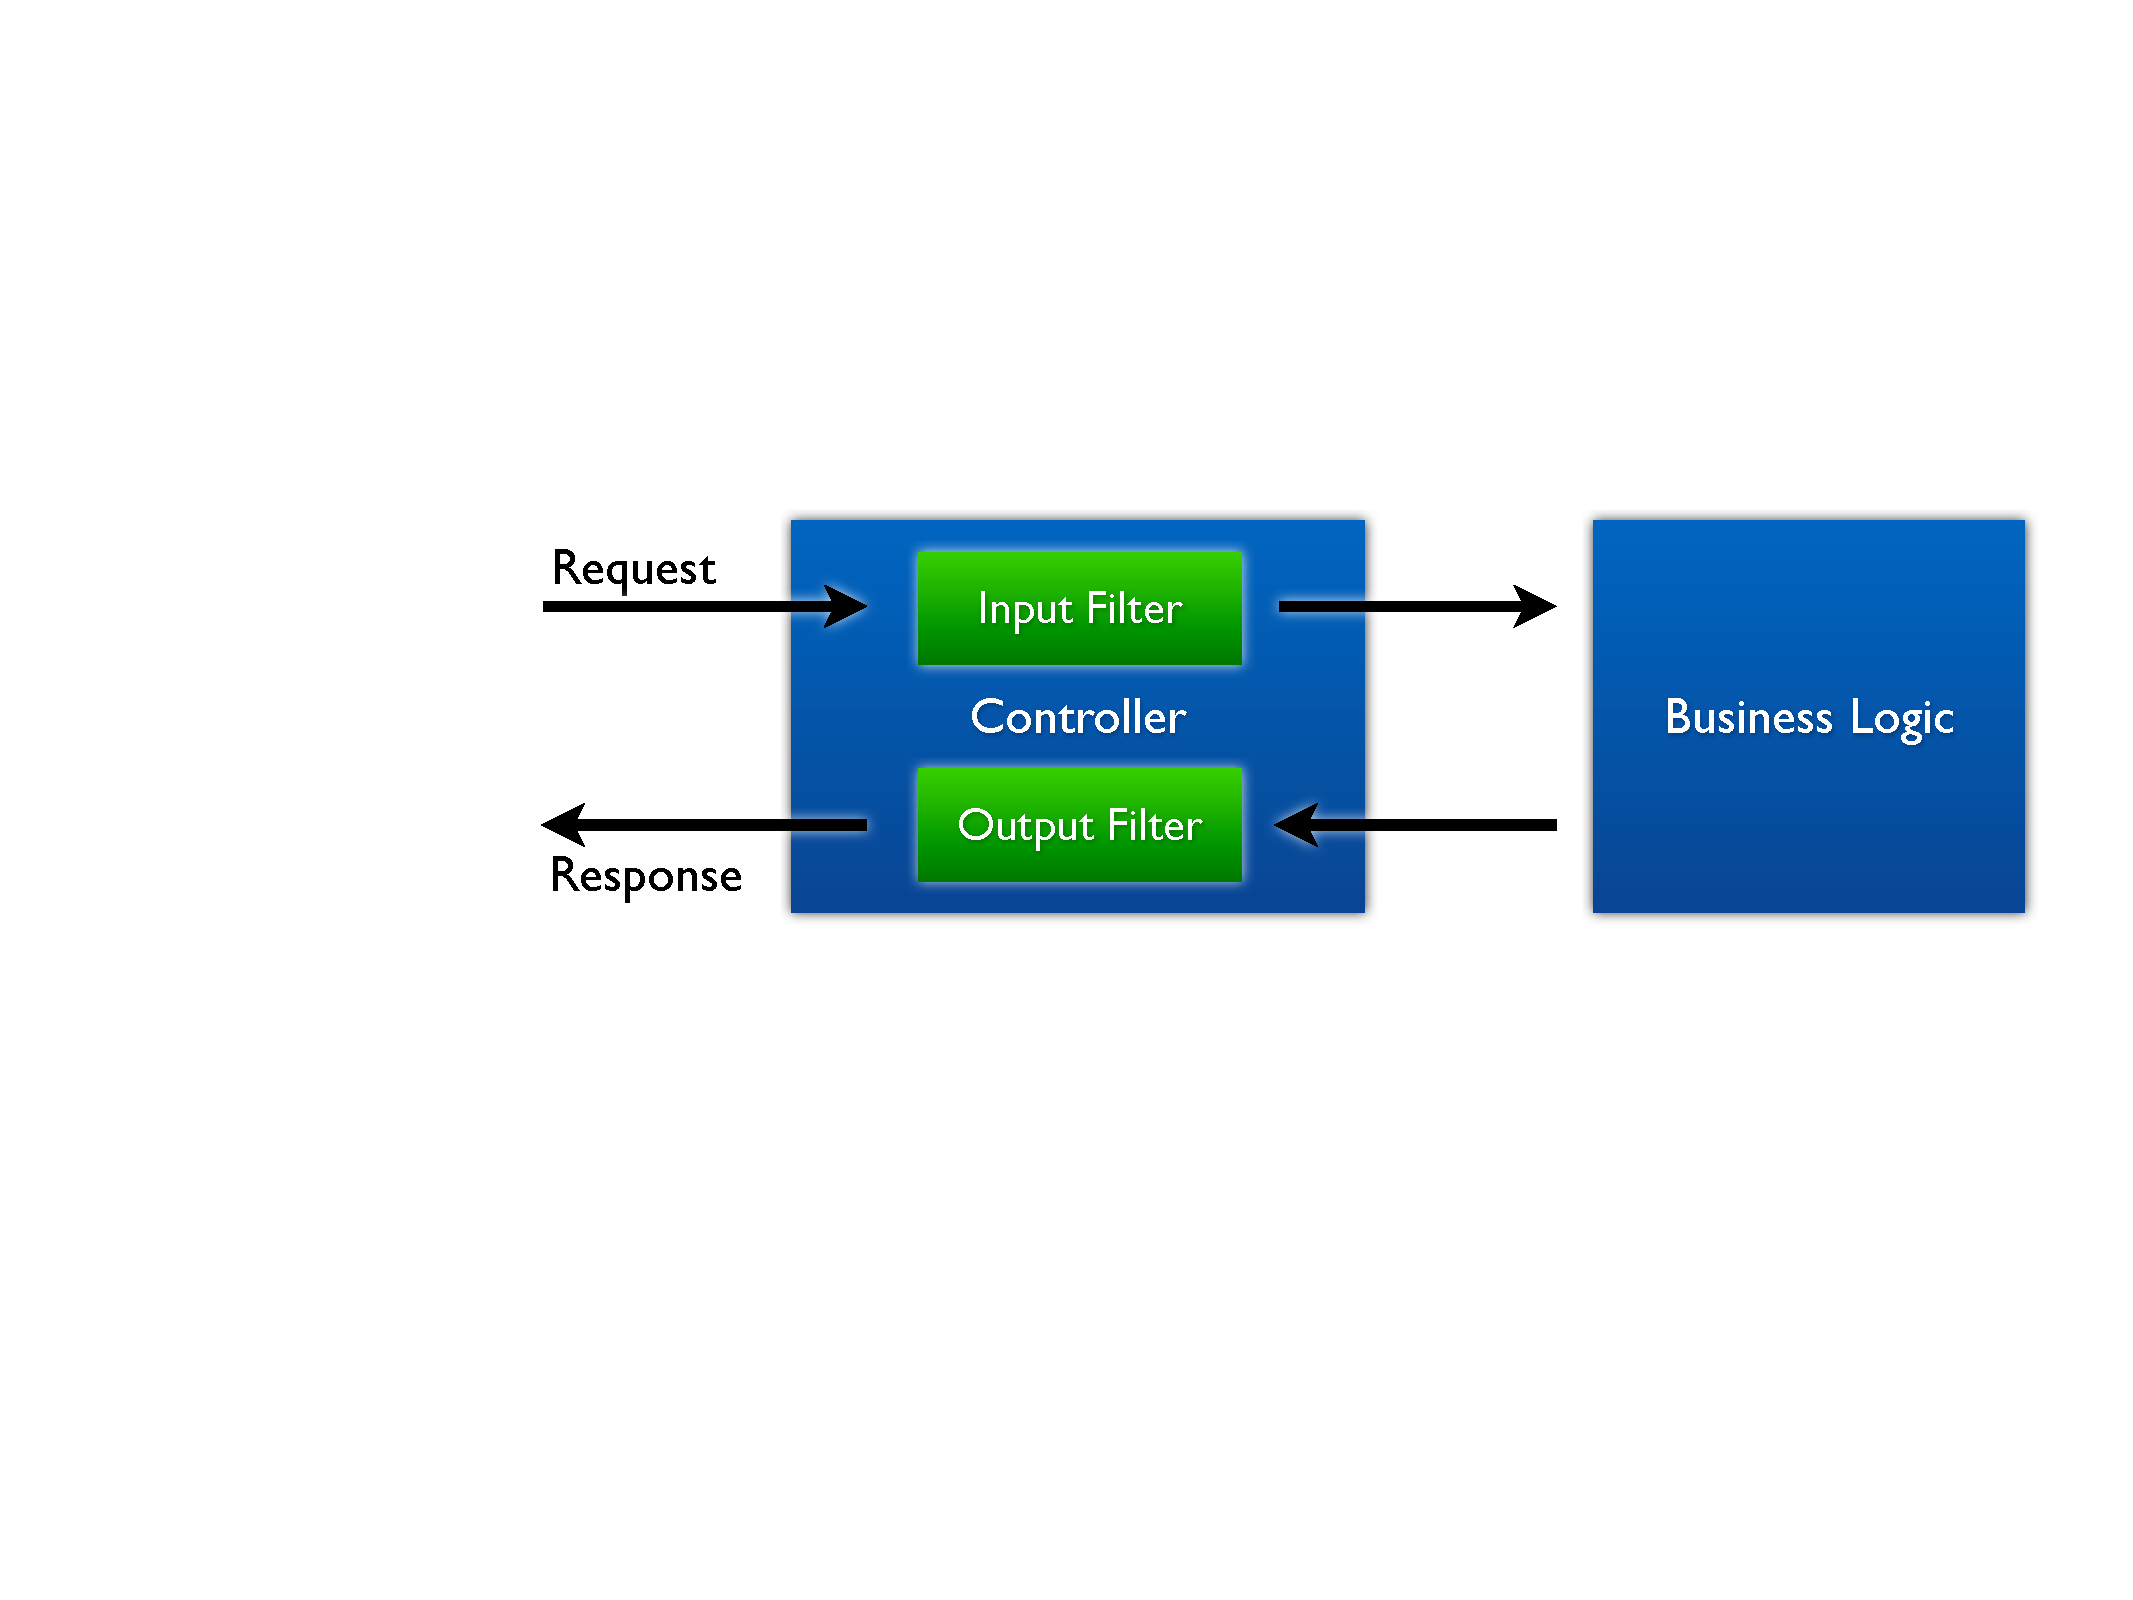
\includegraphics[width=\columnwidth]{images/design_webapplication.pdf}
	\caption{Data flow within our web application.}
	\label{fig:design-web-application}
\end{figure}

Our web application is, as stated in \autoref{sec:architecture}, layered into multiple loosely coupled tiers. Communication between these tiers takes place in strictly specified ways. A request to the system is issued by the user, which directly interacts with the front end through a web browser. It is than processed by a controller, which handles input sanitizing and validating. The controller invokes the business logic which returns structured data (XML in our case). Using XSL-T that data is transforrmed into whatever format is requested and sent back to the front end by the controller.

\begin{description}
\item[Controller] The core of our application is a Servlet according to the Java Servlet Specification. It provides the business layer with session handling and offers access to the data access layer (which is then invoked directly from within the business layer). The main purpose of the Controller is to route data from the front end to the business layer and vice versa. Since no direct access from the front end to the business layer is possible, user privileges are also checked within the controller, so that it is not even possible to pass data to a module of which a user lacks the privilege to make use of.

\item[Modules] To achieve the decoupling of business logic from the controlling unit, we encapsulated it into Modules. These Modules are to be loaded on server startup and provided with an environment; that is, a \emph{RelationManager} for accessing the database. Using Javas Annotation API, the Module classes are provided with information on how the controller should treat them. For example, a method may be annotated with \texttt{@Action}, which declares this method as accessible via the servlet. The Controllers task will then be, to map incoming request to that method. Modules are expected to return a \texttt{org.w3c.dom.Document}\link{http://download.oracle.com/javase/6/docs/api/org/w3c/dom/Document.html}{org.w3c.dom.Document}, which can than be processed by the controller.

\item[OutputConverter] OutputConverter are used for transforming the XML Document which is returned by the business layer into a certain format.

\item[InputConverter] In order to deal with user data, an special mechanism was designed. Data classes which represent forms are provided with declarative information via Annotations. These are to be processed by the Controller to transaprently make the data accessible to the business layer. These form classes are very similar in spirit to Active Records in the data access layer, since they are used to access data as well as transfer data.

\end{description}

\end{multicols}
\begin{multicols}{2}[\subsection{Scheduler algorithm}]

The problem of course scheduling is known to be NP-hard \cite{JSSP}. The course scheduling problem can be approached by using search algorithms. As a matter of fact this works for simple cases only. Course scheduling, especially at universites and similiarly large facilities, goes along with complex constraints. With increasing input and more constraints an optimal solution cannot be computed within a reasonable amount of time. The widely used approach of using a genetic algorithm seemed to be promising and was therefore chosen for our project.

Genetic algorithms are a subset of the metaheuristic optimization algorithms. Metaheuristics, being part of stochastic optimization, are algorithms using randomness to some degree in order to find solutions to hard problems where the solutions are optimal or as optimal as possible. Metaheuristics are applied when little is known about what the optimal solution looks like. Heuristics are hardly useful as neccessary information is lacking. Brute-force is out of question as the space of possible solution is too large. However, when a candidate solution is given it can be rated in order to evaluate how good it is indeed \cite{Luke2009Metaheuristics}.

In order to understand the scheduler algorithm the genetic algorithm operations, \emph{setup}, \emph{fitness function}, \emph{crossover}, \emph{mutate} and \emph{selection}, are best conceived of as core components of the scheduler algorithm. These operations are described below.

\begin{description}
\item[Setup] generates the initial population of candidate solutions in a random or semi-random way. A candidate solution is created when every course is allocated in a room at a given time. The \emph{setup} process is finished when $\lambda$ candidate solutions were created.

\item[Fitness function] rates the candidate solution assigning it a score. The score is mapped to the number of constraints satisfied. The more constraints are satisfied the higher the candidate solution is scored. The score ranges from $0.0$ to $1.0$.

\item[Crossover] creates a new candidate solution by mixing and matching parts of two given candidate solutions. How the mixing and matching is done depends to the representation of a candidate solution. As our representation is a mapping of courses to allocated rooms and times, these allocations are mixed and matched.

\item[Mutation] creates a new candidate solution by taking a given candidate solution and changing a specified amount of course allocations to new, randomly chosen, course allocations.

\item[Selection] iterates the given candidate solutions and keeps only the $\mu$ best solutions. The solutions are selected, according to the score given by the \emph{fitness function}, through dropping the rest of the candidate solutions.
\end{description}

It is also possible that the desired scheduling is not scheduleable at all, for instance when two courses have the hard constraint to be placed at the same room with overlapping time. In this case the scheduling is stopped and the user has to resolve the constraint conflict on their own.

% Figure \ref{fig:schedulercomponents} illustrates the components interaction.

\begin{figure}[H]
	\centering
		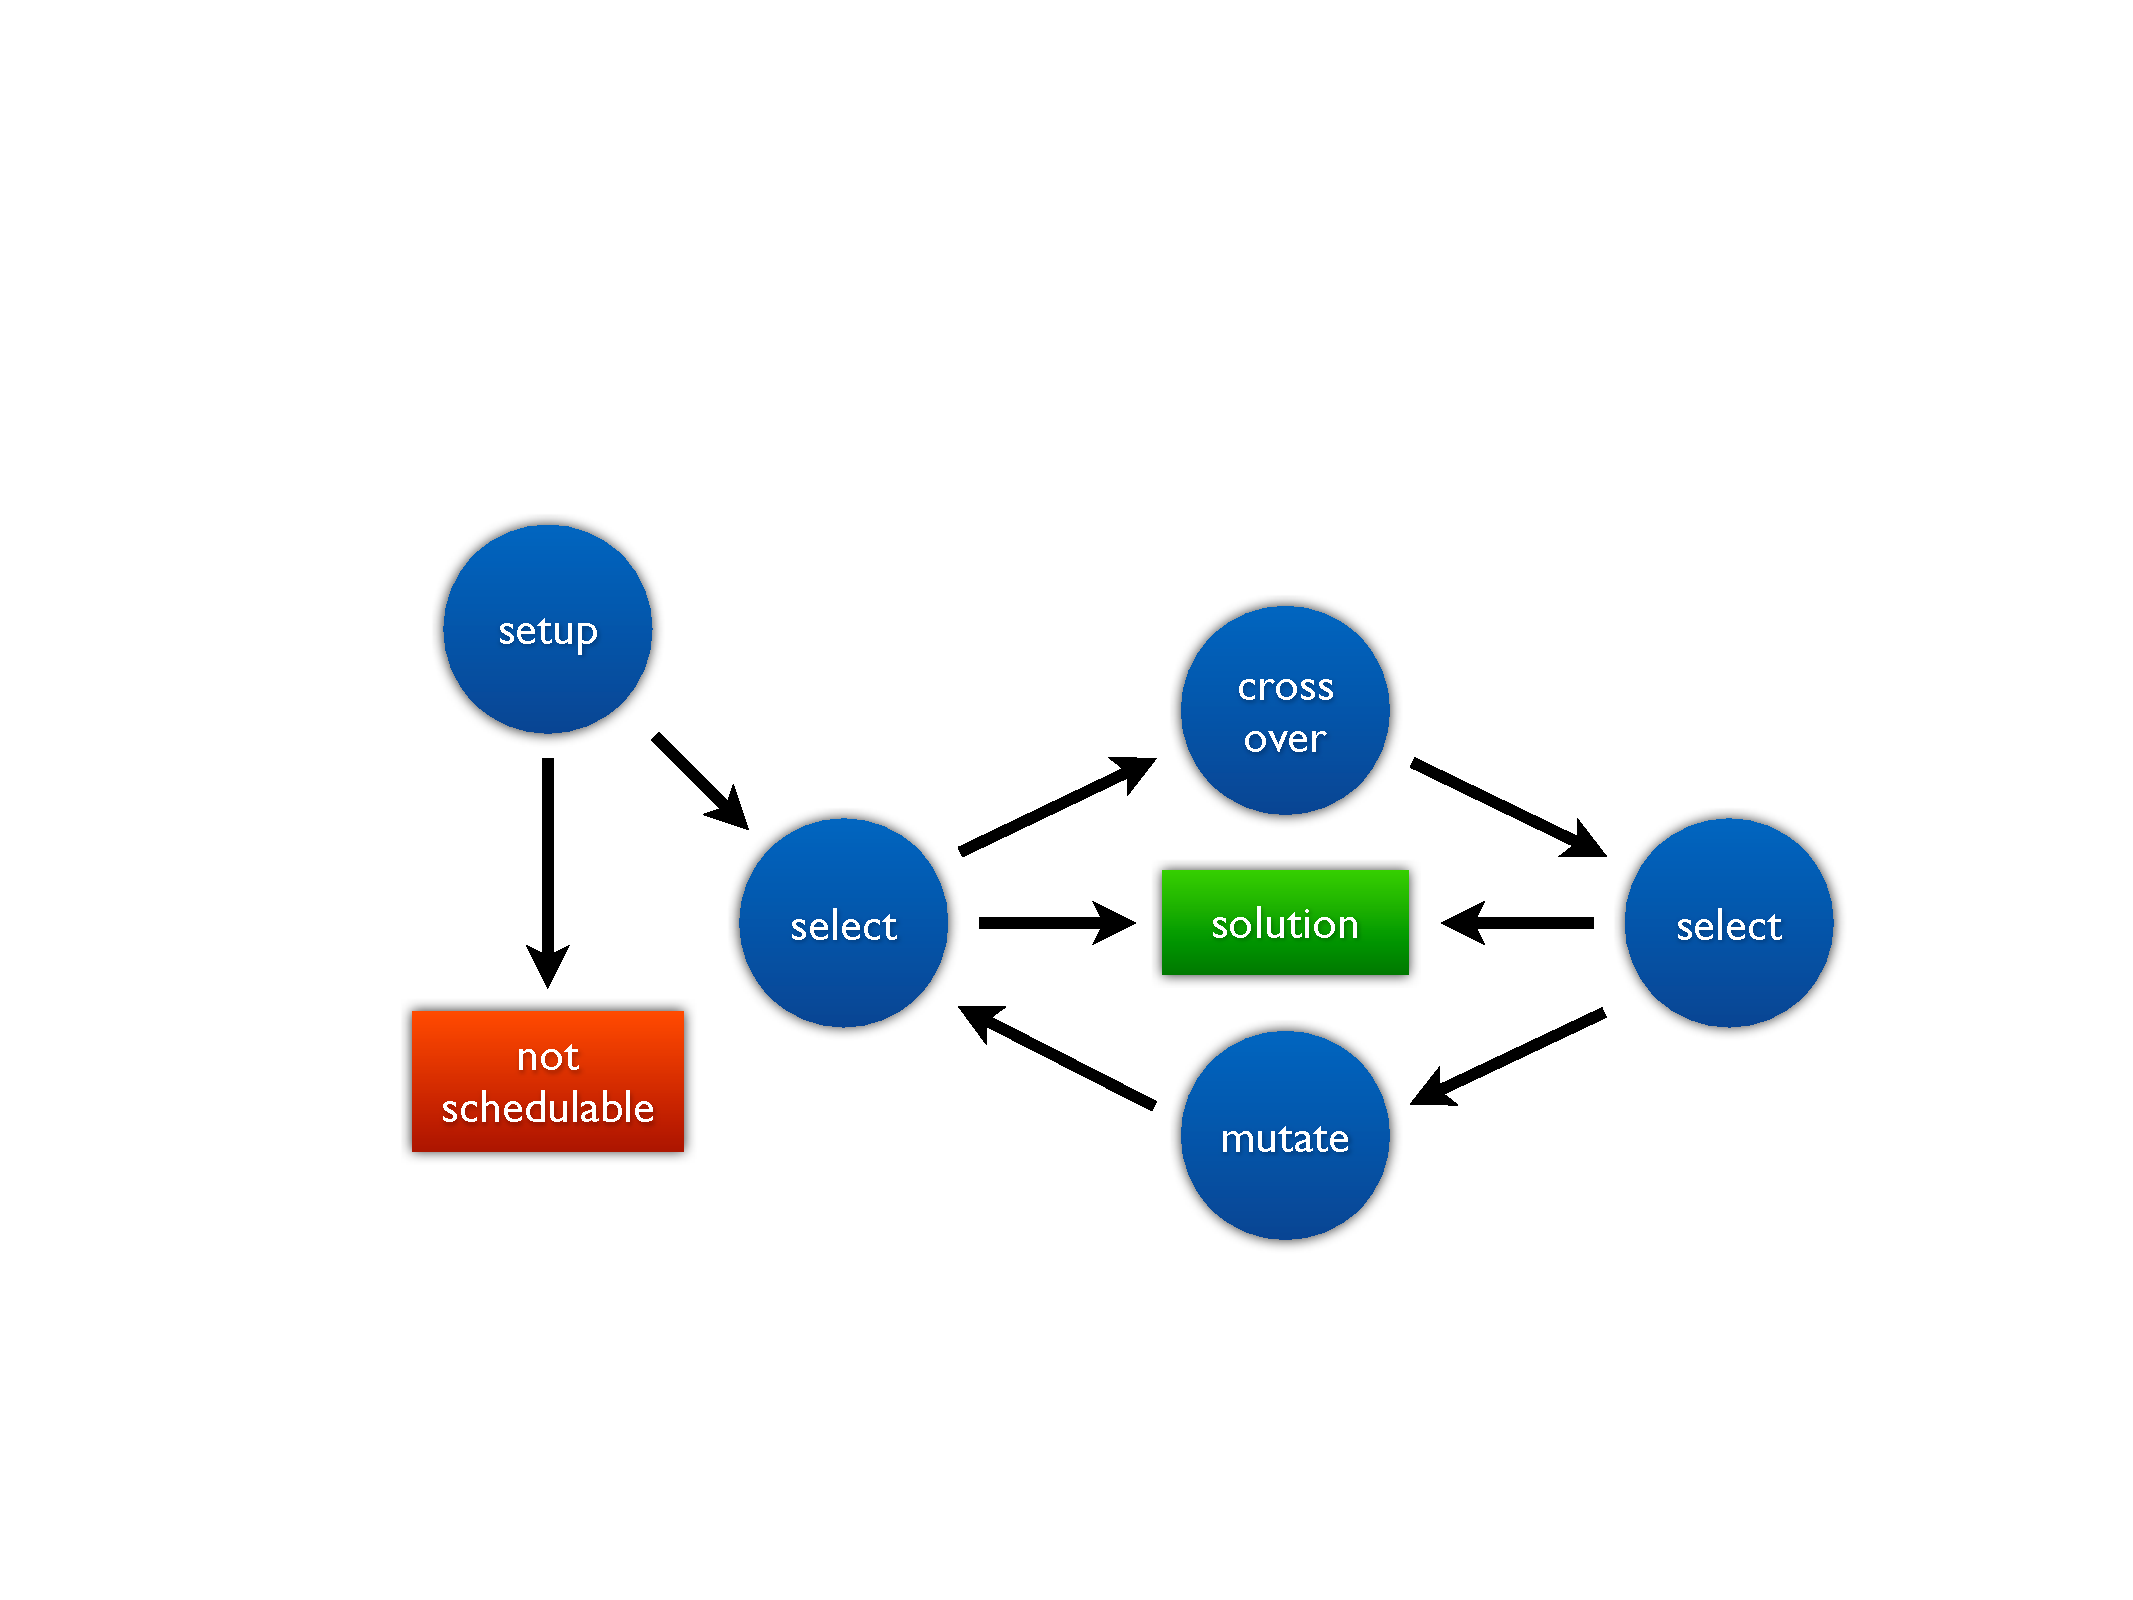
\includegraphics[width=\columnwidth]{images/algorithm.pdf}
	\caption{Routine of the scheduler algorithm. An initial population of candidate solutions is generated. Every candidate solution is rated. If non-solvable conflicts appear the scheduling has to be terminated. Otherwise the setup phase is followed by optimizing the candidate solutions through applying crossover and mutation operations until an optimum schedule is found.}
	\label{fig:schedulercomponents}
\end{figure}

\end{multicols}
\begin{multicols}{2}[\section{Implementation}]
\label{sec:implementation}

The Implementation section covers certain issues regarding implementation tasks. Problems and their solutions will be discussed.


\end{multicols}
\begin{multicols}{2}[\subsection{Data access layer}]

For implementing the data access layer we defined code-templates which were simply filled with values, according to our XML schema definition – much like a serial letter. While tedious in the beginning (since the code-templates are written in XML) we quickly became used to it. Since all classes are built from the same template, it was quite easy fix bugs once and for all.

It also proved to be a quite extendable concept. For example, it took us just a few hours to implement a query cache, which increased the speed of the scheduler about 8 times. Once the API was defined, it was easy to enhance performance without putting the stability of the rest of our code base at risk.

We chose to use Java SEs native SQL-API from the java.sql-package to access the database. Thanks to the use of prepared statements we did not have any trouble with malformed user inputs, making our software virtually invulnerable against things such as SQL injections.

\raggedcolumns
\columnbreak

\paragraph{Use of AspectJ and PL/pgSQL} One of the most compelling features of automatically generating code is, that changes made to the template are reflected in all derived classes. However, it comes at a cost. One can not manually edit that code, without either loosing the advantage of automatically adapting changes or loosing the extensions made manually. Thus we used AspectJ to \emph{cross-cut} the auto-generated classes and so implement special functionality. Using PL/pgSQL these functions were implemented efficiently within the database, taking full advantage of PostgreSQL’s rich set of server-side programming features.

An example for this is the enrollment in courses. To enroll a student into a course (actually a course instance) many requirements have to be checked (whether a user has passed required courses, whether there are enough free seats, etc.). This function was implemented in the database and included into the Java class \emph{CourseInstancce} using an Aspect named \emph{Enrollment}, which introduces the method \emph{enroll(Person p)} in that class.

\paragraph{PostgreSQL-specific issues} The most trouble we had were annoyances and inconsistencies between the promises of the Java SQL API and the implementation of it in the PostgreSQL-JDBC-Driver. For example, \texttt{java.sql.Statement.getGeneratedKeys()} returns any auto-generated keys during the last query. However, the implementation of the PostgreSQL-Driver does not support that feature and so we had to work around this short coming using a PostreSQL-specific language extension.


\end{multicols}
\begin{multicols}{2}[\subsection{Controller}]

In order to implement the Controller and associated interfaces as described in the design section, we had to utilize Javas Reflection API. Problems we faced arose mostly from Javas Type System, especially Generics, which proved to be quite cumbersome to work with.

\paragraph{OutputConverter} Thanks to a clean design it was easier than we thought at first to implement a multitude of different \emph{OutputConverter}. Thus we created a whole lot of them, for XHTML, HTML5 as well as PDF and even text/plain Output.

\paragraph{Shared Code} Since many functions were the same across many different modules in the business layer, we created common abstract classes for shared functionality.


\begin{figure}[H]
	\centering
		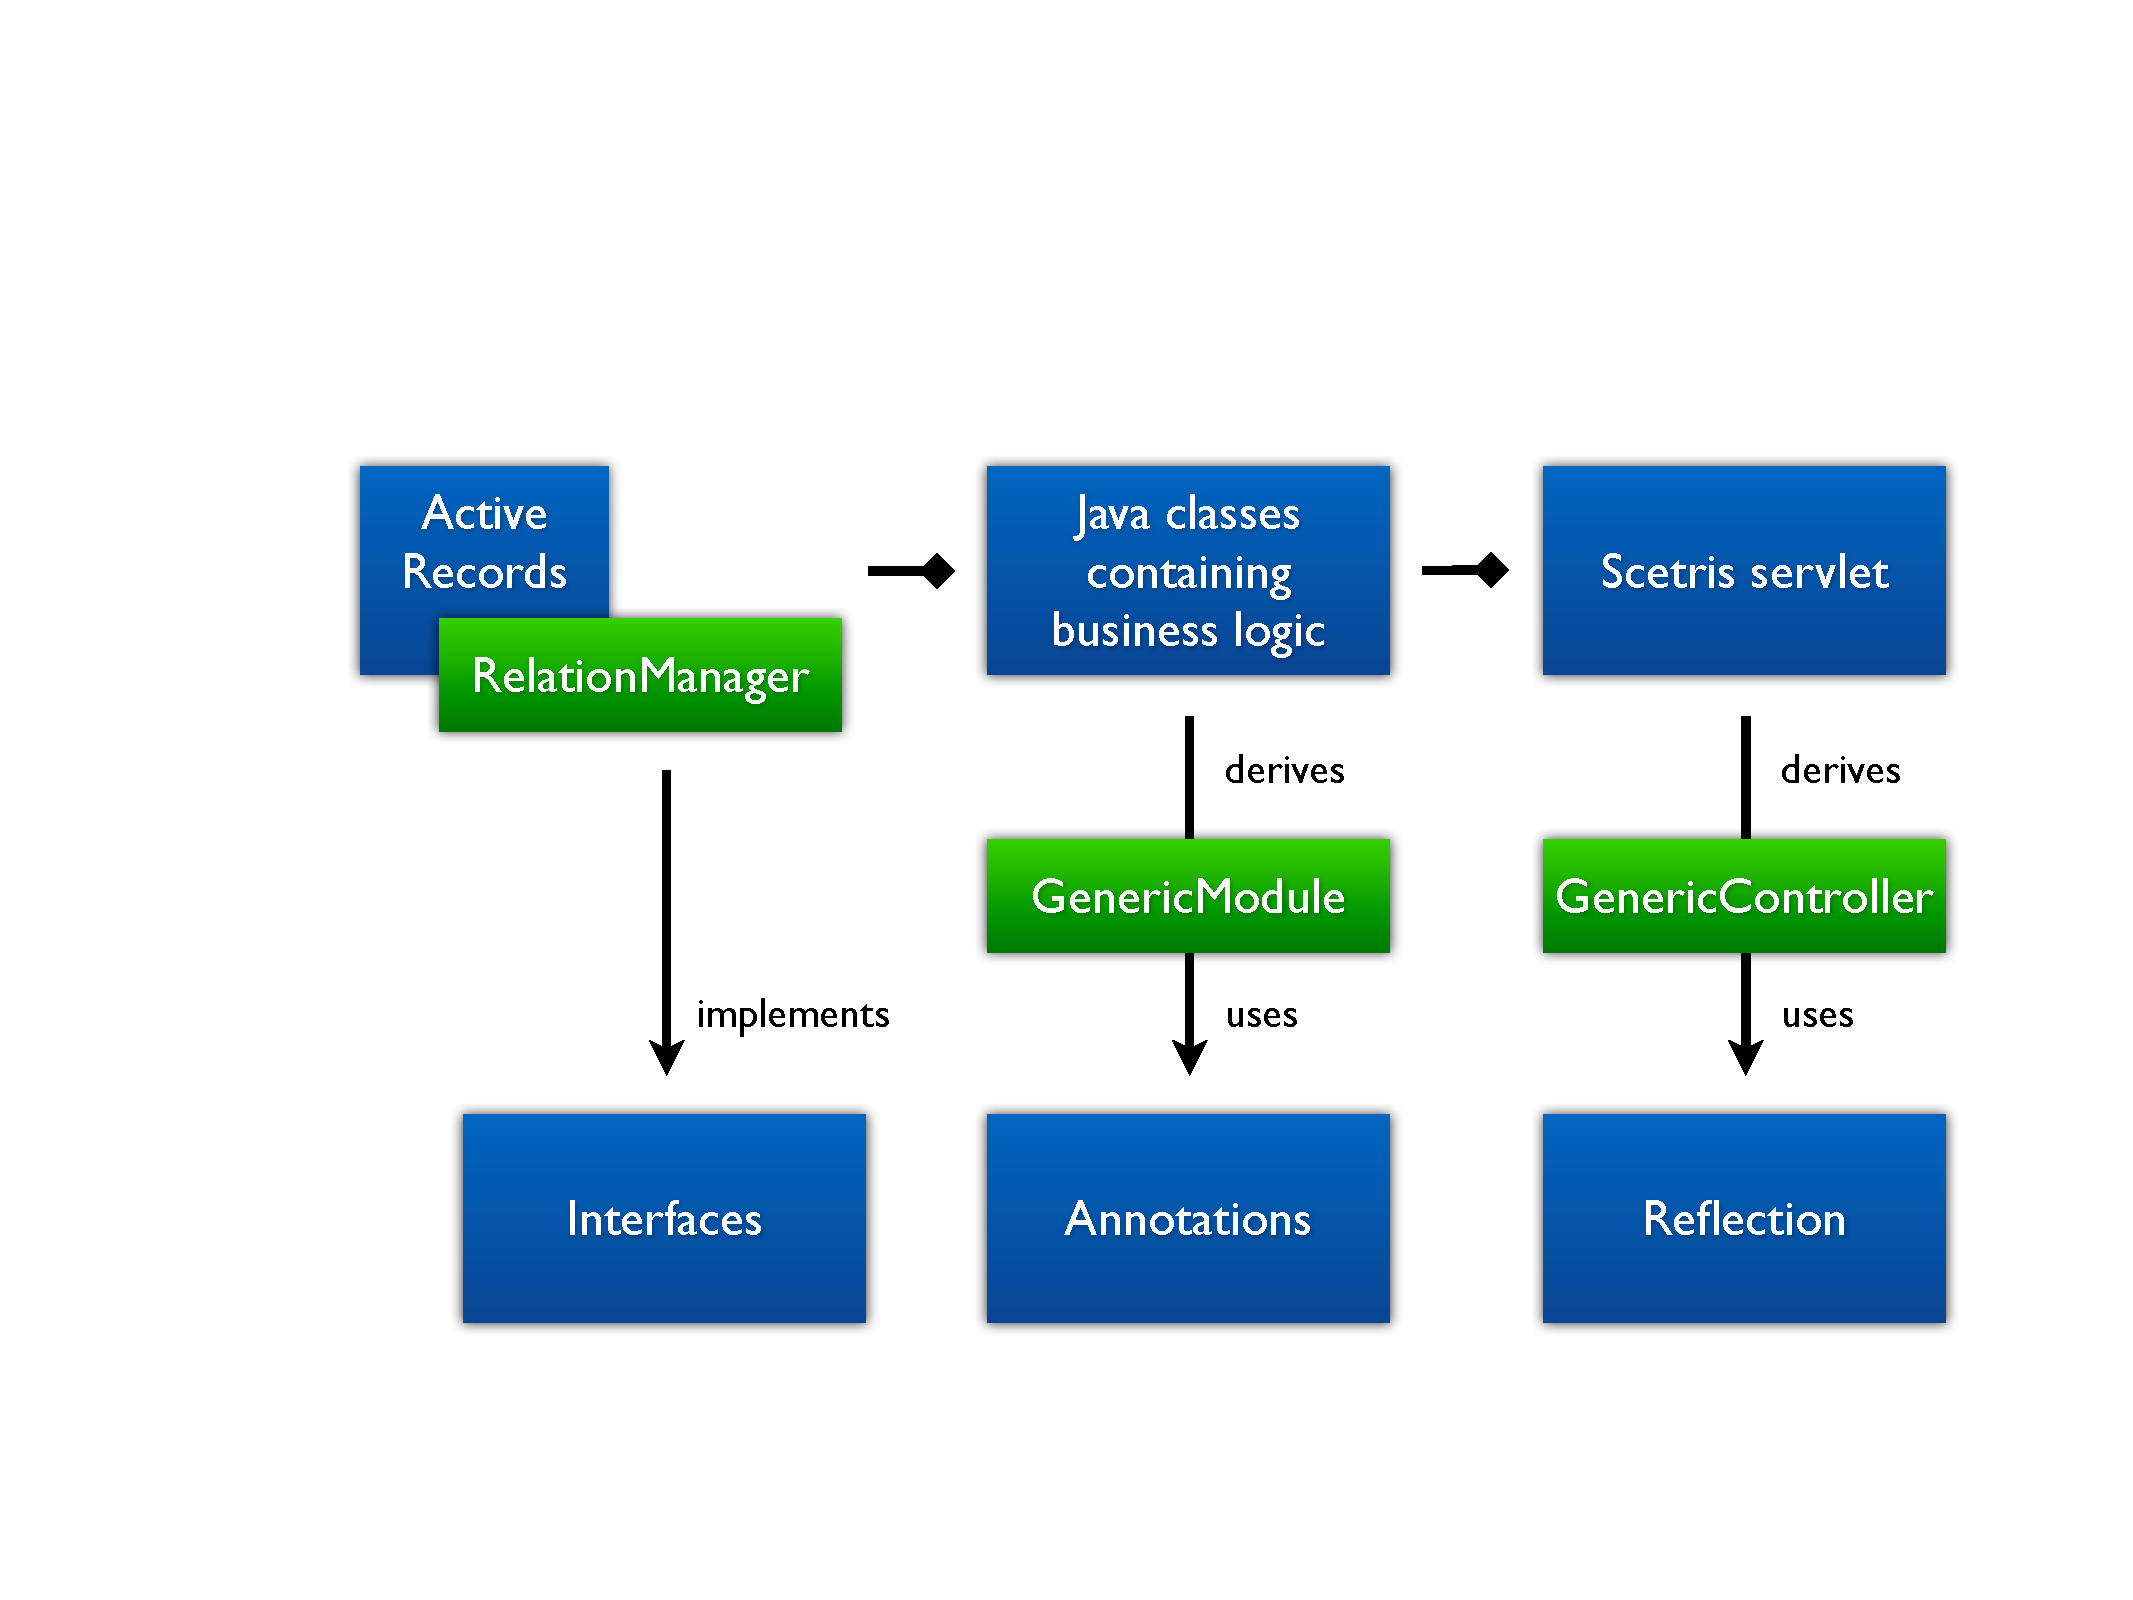
\includegraphics[width=\columnwidth]{images/web-classes.pdf}
	\caption{Composition of business logic, controlling logic and data access layer.}
	\label{fig:scheduler}
\end{figure}


\end{multicols}
\begin{multicols}{2}[\subsection{Front end / Templates}]

The front end was implemented using XSL-T templates. The main idea was to make it easier for us to build the web application. To do so we created lego-bricks -- as we called them -- our main form building mechanism. It simplified the work in a way, that we just handled little data into the templates and got rich, unified forms in return. As a result we did not need to bother about layout and style, since the templates always created HTML which looked similar, thus a uniform look and feel of the site.


\end{multicols}
\begin{multicols}{2}[\subsection{Scheduler}]

The major problem of implementing a genetic algorithm is the question of how to represent the solutions. The genetic algorithm operations presented can only be applied when a fitting data model has been designed. Traditionally an array is used. The \emph{crossover} operation applied on two candidate solutions leads to mixing these values with each other. The \emph{mutation} operation on one candidate solution leads to randomly changing values of the array.

A generic approach to solve this problem is to encode the data model into a byte representation. But since we had chosen AspectJ respectively Java to implement the scheduler we wanted to use the concept of object-orientied programming and all its advantages. Fortunately there was a reference solution\link{http://www.codeproject.com/KB/recipes/GaClassSchedule.aspx}{Homepage of The Code Project with example implementation of genetic algorithm} implemented in C++, which we based our implementation on. The candidate solutions are represented by using a \emph{Map}.

\[CourseElementInstance \mapsto (Room,Time Slot)\]

Every course is mapped to a tuple defined by a room and a time slot. The time slot is the starting time slot of the course [Figure \ref{fig:map}].

\raggedcolumns
\columnbreak

\begin{figure}[H]
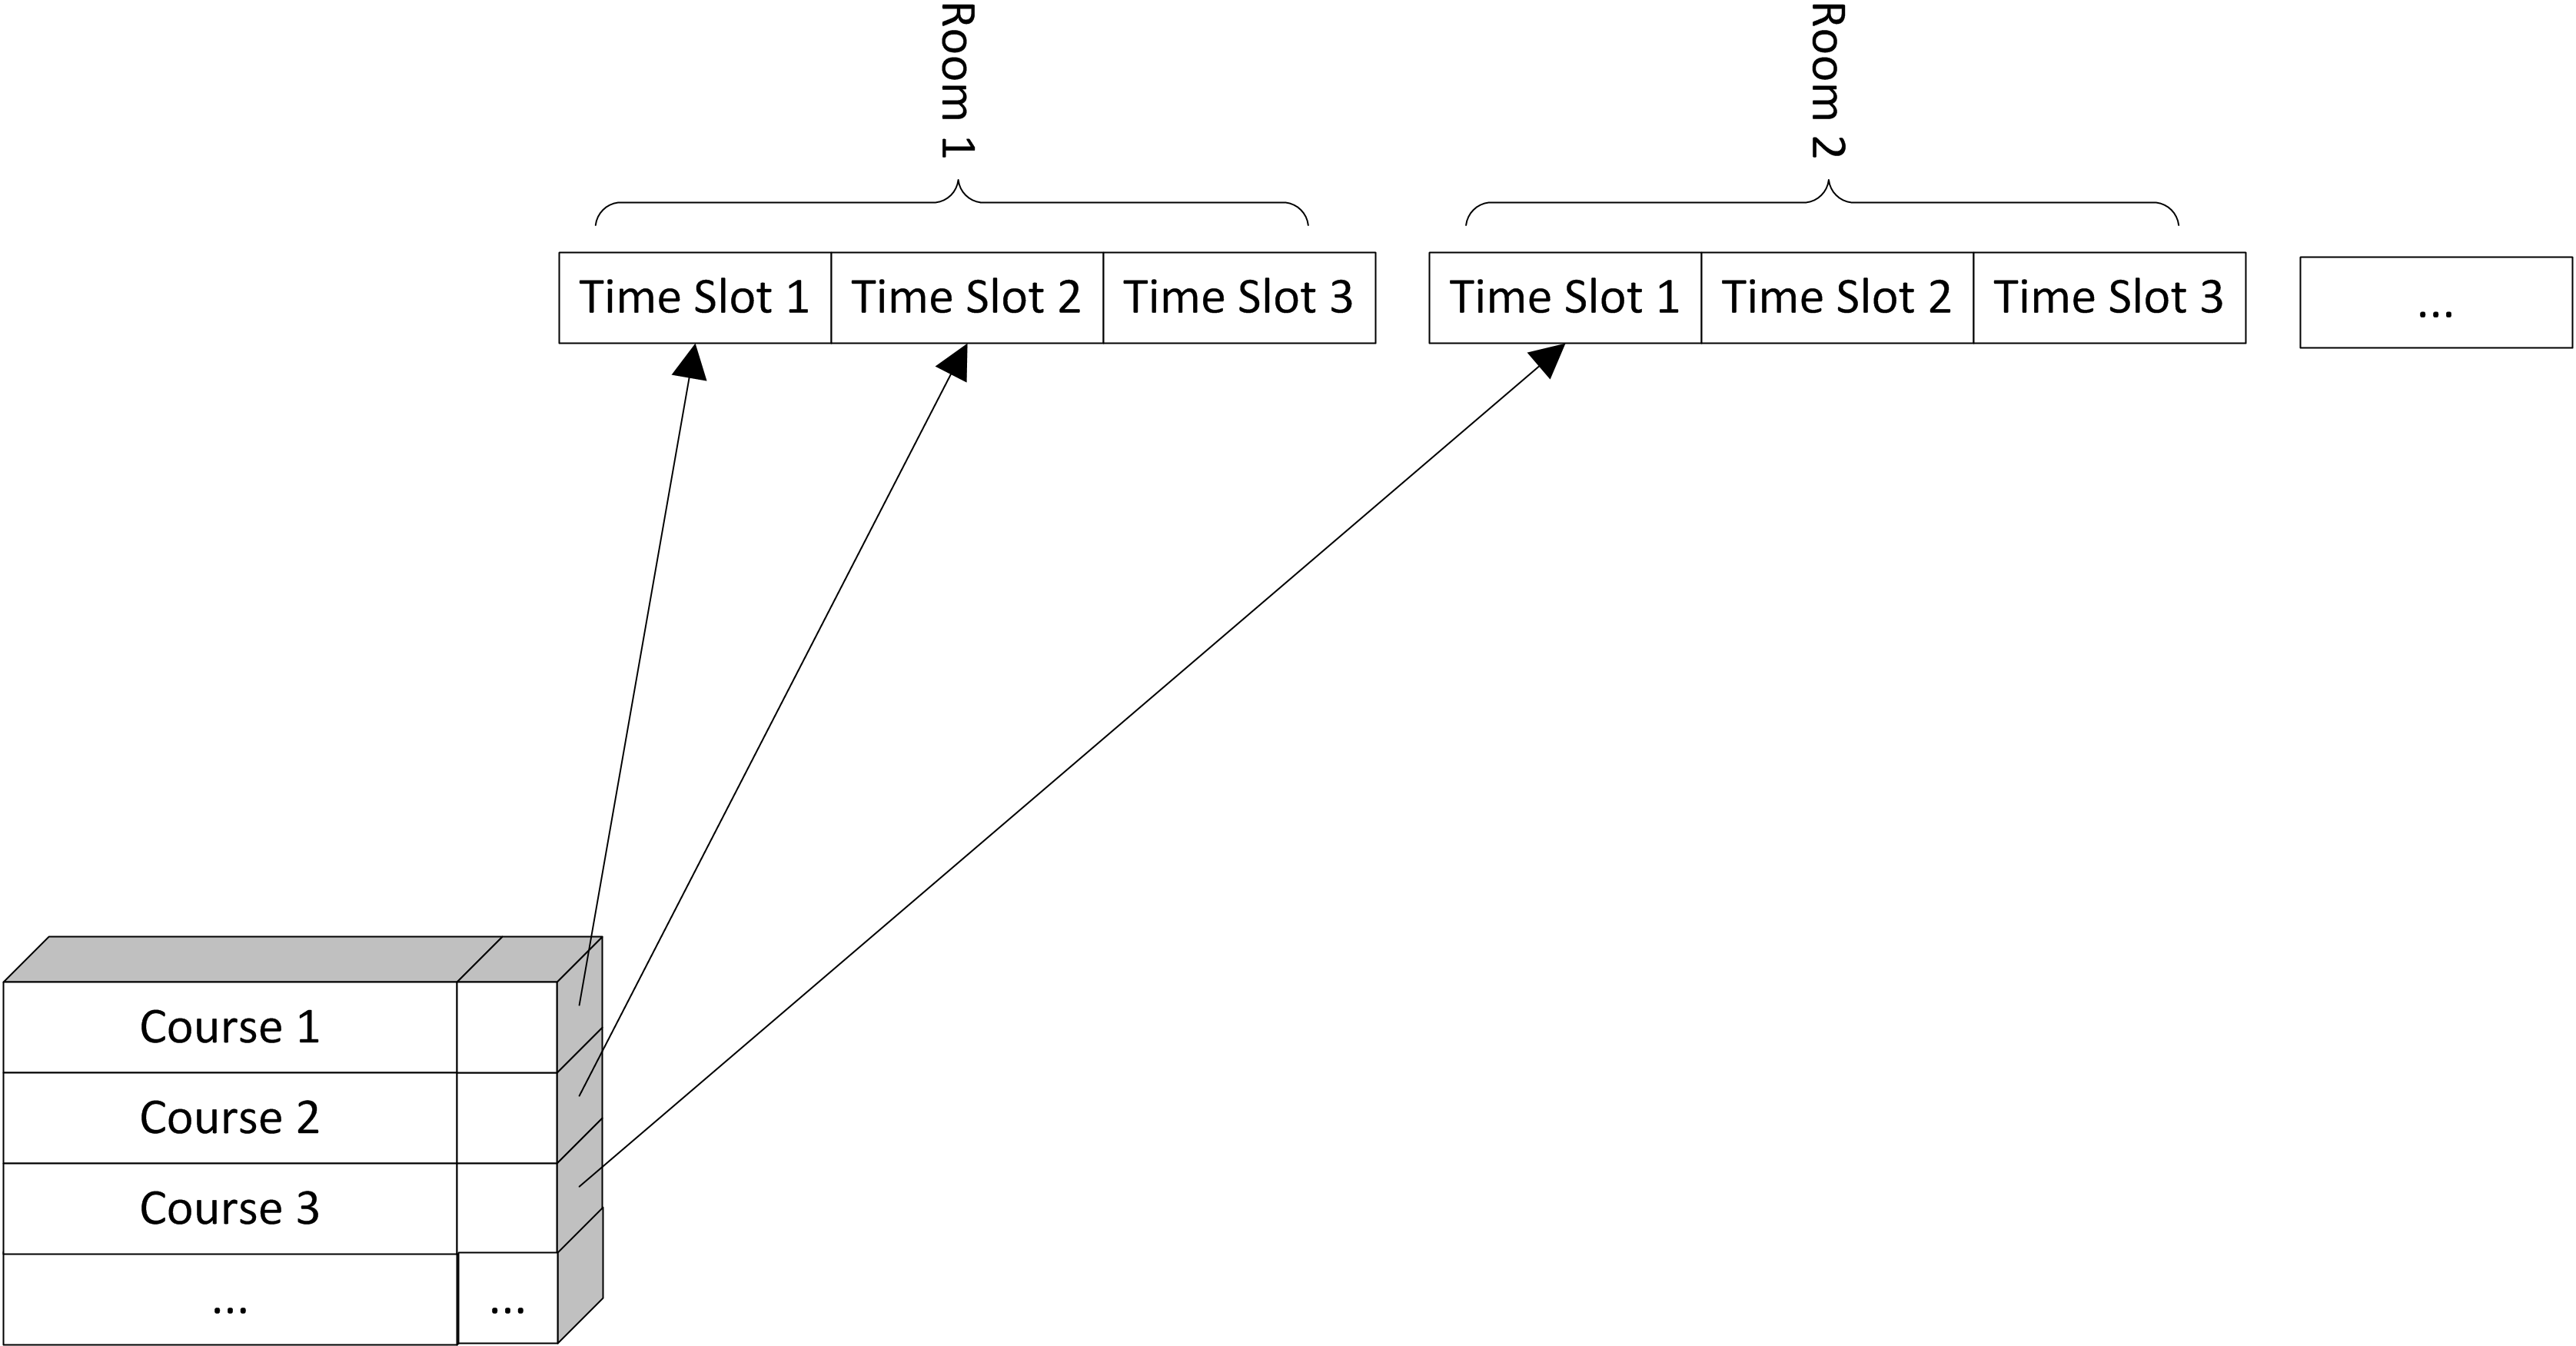
\includegraphics[width=\columnwidth]{images/map.png}%
\caption{Every Course is mapped to a tuple defined by a room and a time slot.}%
\label{fig:map}%
\end{figure}

 As a matter of fact this is not sufficient to model the whole candidate solution. Behind this data model lies another data model modeling the whole timetable. The data model is a list of rooms with each having a further list with time slots. On every time slot there is another list with courses allocated to this position. Instead of a single course a list of courses was chosen because there is the possibility of having one course in the same room at the same time.

\[ [(Room,[(TimeSlot,[CourseElementInstance])] \]

However, applying \emph{crossover} and \emph{mutation} only takes effect on the \emph{Map}. An example of executing \emph{crossover} on the designed data model is illustrated in Figure \ref{fig:data-model}.

\begin{figure}[H]
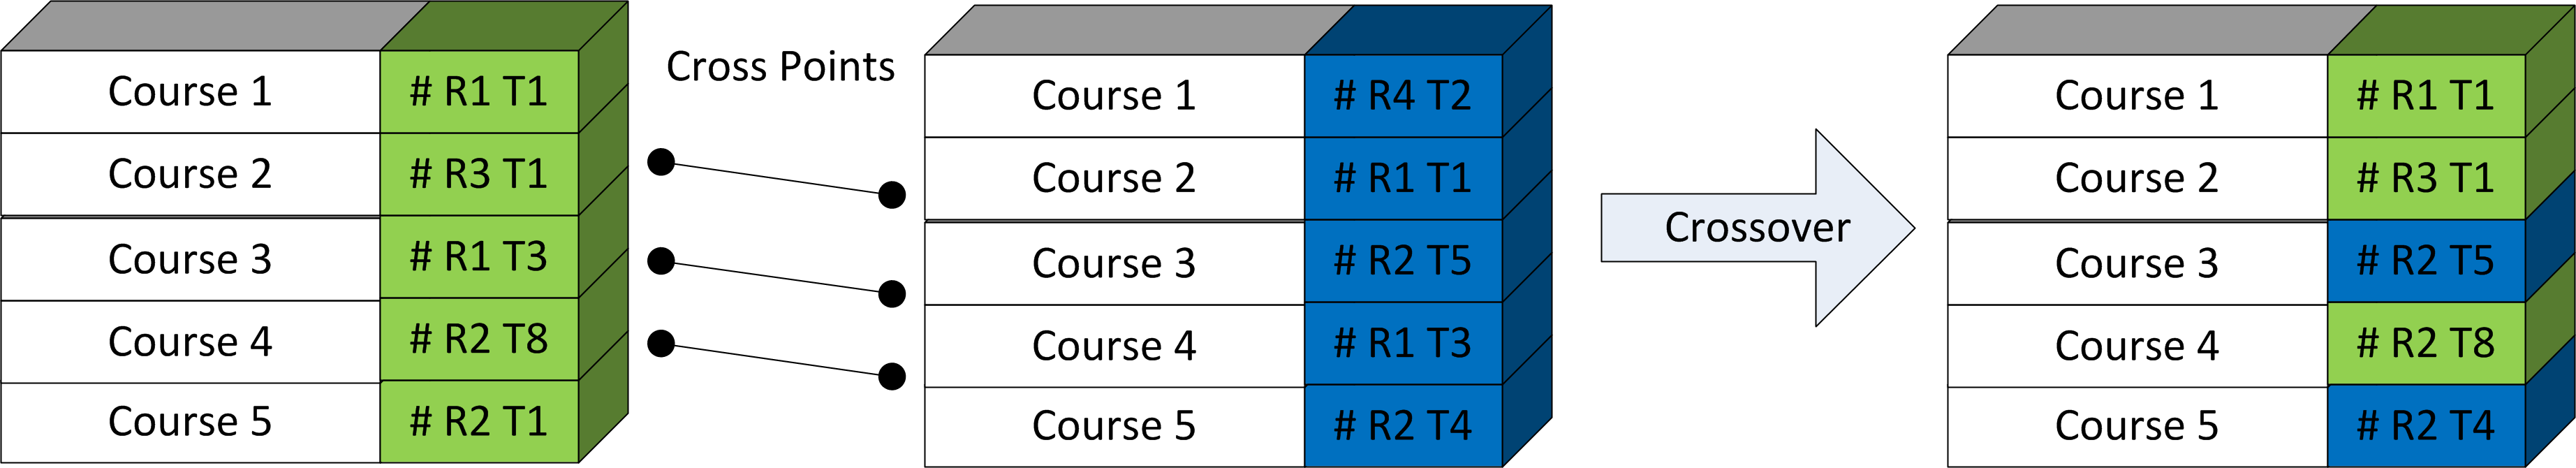
\includegraphics[width=\columnwidth]{images/crossover.png}
\caption{Crossover operation: A specified amount of cross points is chosen randomly. The courses are iterated and taken over to the offspring candidate solution. When a cross point is met the other candidate solution being crossed over is used to take over its course allocations.}
\label{fig:data-model}
\end{figure}

In the implementation phase it turned out using a \emph{setup} allocating the course completely random works for little input very well. With increased input, however, the results by  the classical \emph{setup} lead to quite worse results. These results are supposed to be optimized by the phase of applying \emph{crossover} and \emph{mutate}. As a matter of fact this happens to a certain degree but starts to converge to a certain score.

Therefore an alternative \emph{setup} was implemented. \emph{Greedy setup} combines the approach of a genetic algorithm using metaheuristic with the Greedy algorithm being a subset of the combinatorial algorithm.

\begin{description}
\item[Greedy Setup] generates the initial population of candidate solutions by using a Greedy algorithm. Every course is allocated by placing it to the room which fits its constraints best, for instance the requirement for a specified amount of seats. In order to avoid choosing rooms which exceed the required constraints every room is rated and sorted. In order to avoid overlapping in space and time the courses are placed one after another in the timetable.
\end{description}

There is the possibility of finding an optimal solution in the phase of \emph{Greedy setup}. Therefore the \emph{fitness function} is applied on every generated candidate solution. If an optimal schedule has been found the algorithm terminates.

\end{multicols}
\begin{multicols}{2}[\section{The Application}]

%\emph{Description of our product. Features and the concept behind the UI. Possible improvements and add-ons.}

%\end{multicols}
%\begin{multicols}{2}[\subsection{Usability}]

%\emph{MyCourses} is able to create a semi-automatic scheduling for programs at universities or schools. It can also provide a scheduling that was run fully automatic but the recommended usage is to have \emph{MyCourses} create preliminary versions of a scheduling. These will then be improved by the users via the functionality for collaborative scheduling also provided by \emph{MyCourses}. This process is best used iteratively through several cycles of automatic assignment and manual improvement. To get better results from the automated scheduling users can define requirements and assign those to courses or resources. A requirement that is assigned to a course is regarded as a constraint that either must be met in case of a so called hard-constraint or simply improves the rating of a scheduling in case of a soft-constraint.

All in one the application provides the following functionality (illustration follows)

\begin{itemize}
\item login/logout and get detailed information about your personal profile

\item create, read, delete and modify data related to schedules

\item automatic validation of all forms

\item starting, resuming of schedulings with progress indicator

\item view timetables for a given room, a \emph{CourseInstance} and every user

\item import and export of course-related data

\item view courseinstance data and enroll in them

\item full accessibility on current browsers, even without JavaScript
\end{itemize}
\end{multicols}

\begin{figure}[t]
\setlength\fboxsep{0pt}
\setlength\fboxrule{0.5pt}
\fbox{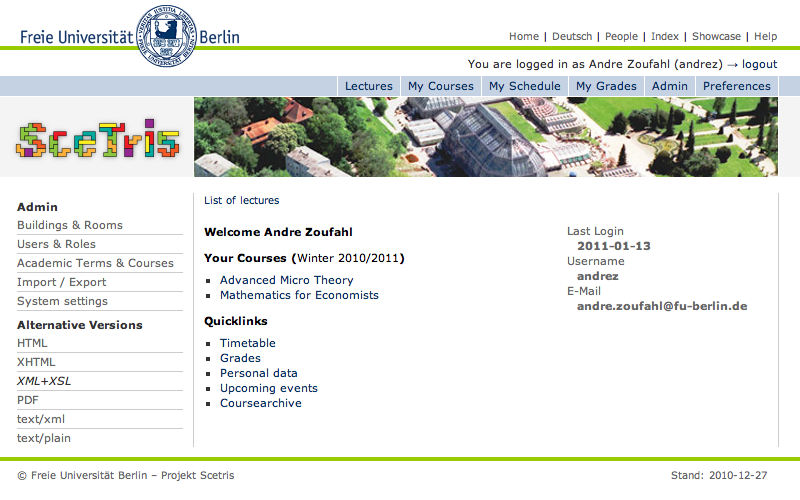
\includegraphics[width=\columnwidth]{images/app/start.png}} 
\caption{Basic layout of our application}%
\end{figure}

\begin{multicols}{2}

\begin{figure}[H]
\fbox{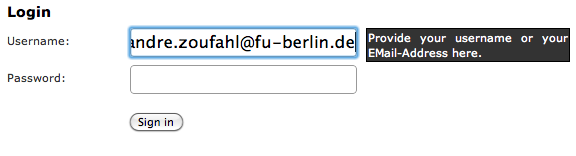
\includegraphics[width=\columnwidth]{images/app/login.png}}%
\caption{Login: input fields provide user with information on what to fill in}%
\end{figure}

\begin{figure}[H]
\fbox{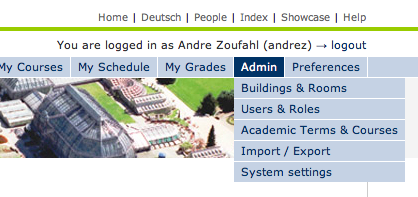
\includegraphics[width=\columnwidth]{images/app/login_after.png}}%
\caption{Login status is tracked on every page. Navigation provides submenus when hovering over items.}%
\end{figure}

\end{multicols}
\begin{multicols}{2}

\begin{figure}[H]
\fbox{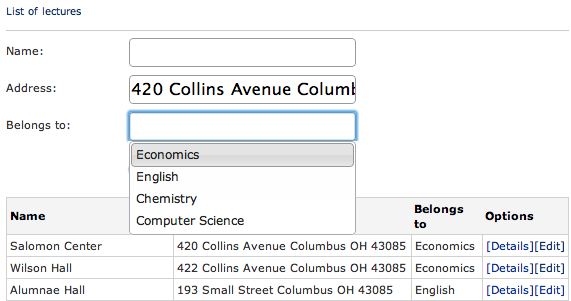
\includegraphics[width=\columnwidth]{images/app/building_list.png}}%
\caption{With JavaScript activated selections morph into textfields with automatic proposals.}%
\end{figure}

\begin{figure}[H]
\fbox{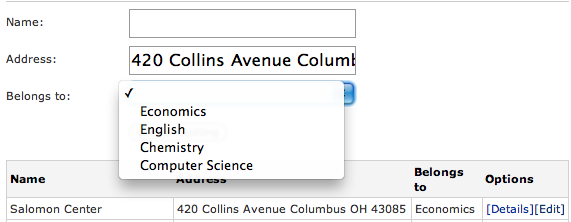
\includegraphics[width=\columnwidth]{images/app/building_list_nojs.png}}%
\caption{Without JavaScript the standard selection is used.}%
\end{figure}

\end{multicols}
\begin{multicols}{2}

\begin{figure}[H]
\fbox{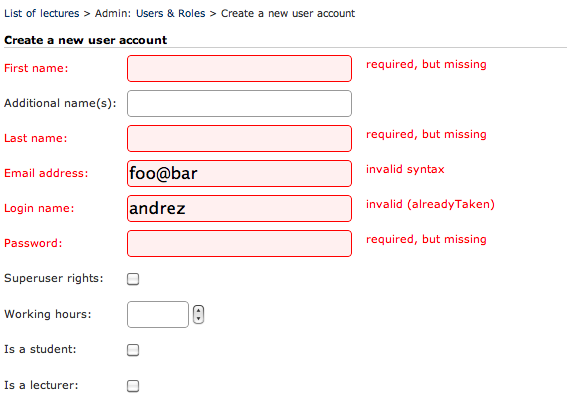
\includegraphics[width=\columnwidth]{images/app/forms_invalid.png}}%
\caption{Form validation: no data can be send until all problems were solved.}%
\end{figure}

\begin{figure}[H]
\fbox{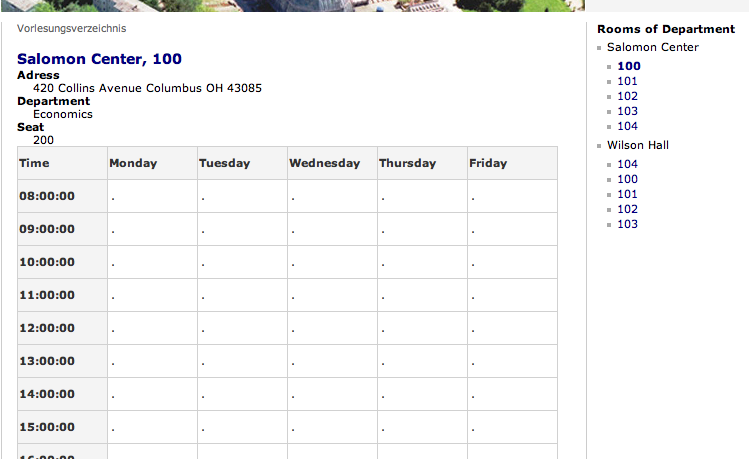
\includegraphics[width=\columnwidth]{images/app/timetable_empty.png}}%
\caption{Before scheduling: CourseElementInstances have no time or room assigned, all rooms are free.}%
\end{figure}

\end{multicols}
\begin{multicols}{2}

\begin{figure}[H]
\fbox{
\includegraphics[width=\columnwidth]{images/app/scheduler_start.png}}%
\caption{If the scheduler is not running, it's possible to schedule the academic term for a given department.}%
\end{figure}

\begin{figure}[H]
\fbox{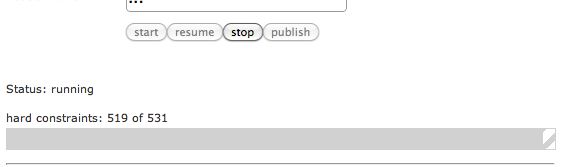
\includegraphics[width=\columnwidth]{images/app/scheduler_running.png}}%
\caption{A progress bar indicates how many constraints are already solved.}%
\end{figure}

\end{multicols}
\begin{multicols}{2}

\begin{figure}[H]
\fbox{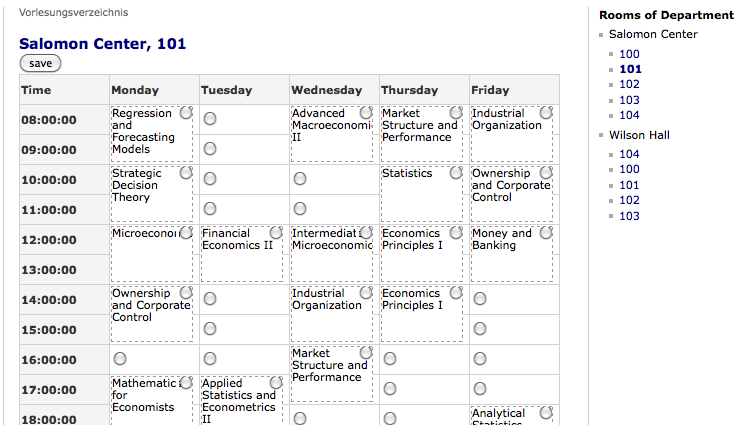
\includegraphics[width=\columnwidth]{images/app/timetable_edit.png}}%
\caption{Manual changes: after scheduling the program manager can also swap positions of courses.}%
\end{figure}

\begin{figure}[H]
\fbox{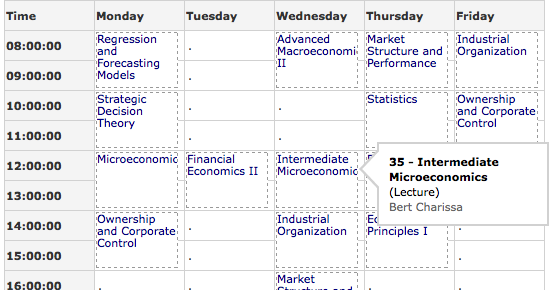
\includegraphics[width=\columnwidth]{images/app/timetable_final.png}}%
\caption{After scheduling: every room contains several CourseElementInstances. Hovering over an event provides the user with data about the event as well as a direct link to the related CourseInstance.}%
\end{figure}

\end{multicols}
\pagebreak
\begin{multicols}{2}

\begin{figure}[H]
\fbox{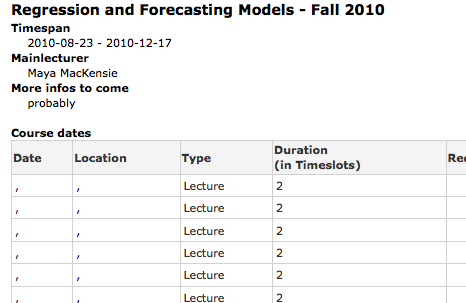
\includegraphics[width=\columnwidth]{images/app/coursedetail_empty.png}}%
\caption{Before publishing of the scheduling every CourseInstance may be inspected but has no dates for their CourseElementInstances.}%
\end{figure}

\begin{figure}[H]
\fbox{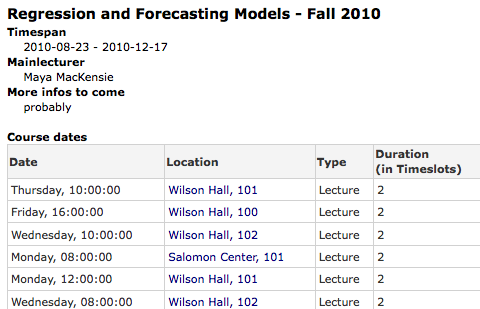
\includegraphics[width=\columnwidth]{images/app/coursedetail_published.png}}%
\caption{After the program manager published and freezed the scheduling it is possible to enroll on any given CourseInstance.}%
\end{figure}

\end{multicols}
\begin{multicols}{2}

\begin{figure}[H]
\fbox{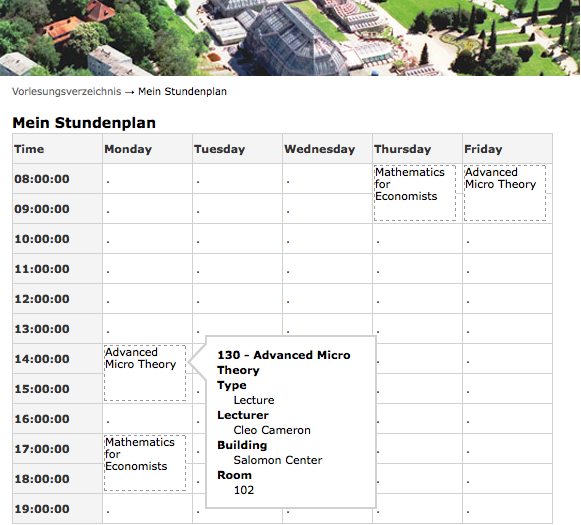
\includegraphics[width=\columnwidth]{images/app/mytimetable.png}}%
\caption{Once the user enrolls in some CourseInstances the user can view its personal timetable for the week.}%
\end{figure}

\end{multicols}
\begin{multicols}{2}[\section{Verification and validation}]
\label{sec:verification-and-validation}

This section will cover testing and other measurements which were taken to reassure ourselves of the correctness of our implementations. However, performance measurement is also part of verification and validation.

\end{multicols}
\begin{multicols}{2}[\subsection{Unit tests using JUnit and automated testing using Cobertura}]

In order to test the correctness of \emph{MyCourses} we applied JUnit. Additonally we used Cobertura to check the code and branch coverage of each unit test. Since total code or even branch coverage was a too time intense task, we decided to concentrate the unit tests on only the most important parts of \emph{MyCourses}. This encompass unit testing for the scheduler and the complete data access layer where the tasks are most critical.

Testing the scheduler for correctness is a non-trivial task. Not only does the presence of a genetic algorithm increase the complexity, but its random-factor also makes it hard to test conditions which have to be satisfied at all times. One approach to improve the testability of the scheduler is the introduction of a seeded random generator. Whenever randomness is applied in the scheduler, it can be reproduced by using the same seed.

In order to achieve a high guarantee of the schedulers correctness JUnit tests were implemented as fine-granular as possible. This implies unit tests for every component of the scheduler. Unfortunately, unit tests allow only little input testing. Data-driven testing is a more promising approach for testing the scheduler.

As we were in need of real world tests we wrote a test data generator. Data sets were entered from the New York University\link{http://www.nyu.edu}{New York University} Course Schedule Search\link{http://www.nyu.edu/registrar/listings/}{New York University Course Schedule Search}.

\end{multicols}
\begin{multicols}{2}[\subsection{Performance and Benchmarking}]

Performance, especially of the scheduler, can be easily tested by test runs with varying size of data input. However this gives no detailed information about the actual performance of separate components. For that reason the profiler \ads{JProfiler} was used to inspect the Java Virtual Machine while executing the program.

This lead to a step-by-step process of picking up the slowest component display in the profiler and trying to improve its performance. In some cases this procedure gave us huge performance boosts.

A weak point of the scheduling performance was the rating of candidate solutions. When checking the constraint satisfactions many data sets have to be queried. The emerging I/O blocking slows the scheduler down. We coped with this task by introducting a query cache.

Also we provided a benchmark of our own, which runs the scheduler with different seeds and different configurations regarding the algorithm and regarding the size of the data sets. For instance the department \emph{Economics} has the following data to be scheduled:

\vskip 2ex

\begin{tabular}{lc}
Courses: & 43\\
CourseElements: & 62\\
CourseInstances: & 43\\
CourseElementInstances: & 181\\
\end{tabular}

\vskip 2ex

Without further constraints, but the default constraints \emph{not more then 1 course in the same room at the same time} and \emph{the course lecturer teaches no course at the same time}, the computation is often done in less than 15 minutes.

However, with the increase of custom hard and soft constraints the probability of finding an optimal schedule in a reasonable time decreases dramatically. To some extend the optimization done by the genetic algorithm depends on luck solving remaining conflicts.

But as the scheduler provides a fair pre-schedule we give the responsibility to the user solving remaining conflicts.
\end{multicols}
\begin{multicols}{2}[\section{Outcomes \& lessons learned}]
\label{sec:outcomes}

For all of us this was the first project of this dimension and duration. We took the chance to put into practice what we had learned in our software engineering course – in particular going through the whole software development cycle. We found that project oriented approaches are hard to adhere to in an educational setting. Our team could not meet as often as we wanted and our studies interferred much more with our project than we had imagined.

Thus, working on a project like this one was a very challenging task. Sometimes it was frustrating to keep working on the project, due to slow progress or heavy workload. But, it was also a very exciting experience. We could not only learn about many technologies we previously did not know, but we also learned a lot about ourselves and about team work. We experienced that we are very different people with different approaches to problems. Everyone learned to get along with the idiosyncracies of the others.

In particular we learned how to develop software collaboratively and maintain a large code base. We learned a lot about configuration management, build process automatization, web development, and unit testing, which are all topics which we heard about at our university but never got to excercise in practice. We recognized how it is not always easy to write unit tests instead of implementing features as there is the feeling of stalling progress.

Since all of this was a new domain for us, we did not manage to stick to our plan, often due to goals that were set too high to begin with. We realized how important it is to meet regularly and how hard it is to coordinate a group of just five students. The meetings had the the strongest effect on the team. While discussing problems and comparing work results we have learned to give constructive feedback to each other. It is now clear to us, that honesty and respect have a great impact on the success of a team.

However we managed to fulfill the major requirements. We are content with what we achieved, since we did have a lot of fun and the final application is a stable and well working piece of software.



\end{multicols}
\begin{multicols}{2}

\nocite{*}
\bibliographystyle{plain}
\pdfbookmark[1]{References}{bib}
\bibliography{summary_report}

\begin{figure}[H]

\includegraphics[width=\columnwidth]{images/hack_whitespace.png}
\end{figure}

\end{multicols}

\end{document}
